% Options for packages loaded elsewhere
\PassOptionsToPackage{unicode}{hyperref}
\PassOptionsToPackage{hyphens}{url}
\PassOptionsToPackage{dvipsnames,svgnames,x11names}{xcolor}
%
\documentclass[
  letterpaper,
  DIV=11,
  numbers=noendperiod]{scrartcl}

\usepackage{amsmath,amssymb}
\usepackage{lmodern}
\usepackage{iftex}
\ifPDFTeX
  \usepackage[T1]{fontenc}
  \usepackage[utf8]{inputenc}
  \usepackage{textcomp} % provide euro and other symbols
\else % if luatex or xetex
  \usepackage{unicode-math}
  \defaultfontfeatures{Scale=MatchLowercase}
  \defaultfontfeatures[\rmfamily]{Ligatures=TeX,Scale=1}
\fi
% Use upquote if available, for straight quotes in verbatim environments
\IfFileExists{upquote.sty}{\usepackage{upquote}}{}
\IfFileExists{microtype.sty}{% use microtype if available
  \usepackage[]{microtype}
  \UseMicrotypeSet[protrusion]{basicmath} % disable protrusion for tt fonts
}{}
\makeatletter
\@ifundefined{KOMAClassName}{% if non-KOMA class
  \IfFileExists{parskip.sty}{%
    \usepackage{parskip}
  }{% else
    \setlength{\parindent}{0pt}
    \setlength{\parskip}{6pt plus 2pt minus 1pt}}
}{% if KOMA class
  \KOMAoptions{parskip=half}}
\makeatother
\usepackage{xcolor}
\setlength{\emergencystretch}{3em} % prevent overfull lines
\setcounter{secnumdepth}{-\maxdimen} % remove section numbering
% Make \paragraph and \subparagraph free-standing
\ifx\paragraph\undefined\else
  \let\oldparagraph\paragraph
  \renewcommand{\paragraph}[1]{\oldparagraph{#1}\mbox{}}
\fi
\ifx\subparagraph\undefined\else
  \let\oldsubparagraph\subparagraph
  \renewcommand{\subparagraph}[1]{\oldsubparagraph{#1}\mbox{}}
\fi


\providecommand{\tightlist}{%
  \setlength{\itemsep}{0pt}\setlength{\parskip}{0pt}}\usepackage{longtable,booktabs,array}
\usepackage{calc} % for calculating minipage widths
% Correct order of tables after \paragraph or \subparagraph
\usepackage{etoolbox}
\makeatletter
\patchcmd\longtable{\par}{\if@noskipsec\mbox{}\fi\par}{}{}
\makeatother
% Allow footnotes in longtable head/foot
\IfFileExists{footnotehyper.sty}{\usepackage{footnotehyper}}{\usepackage{footnote}}
\makesavenoteenv{longtable}
\usepackage{graphicx}
\makeatletter
\def\maxwidth{\ifdim\Gin@nat@width>\linewidth\linewidth\else\Gin@nat@width\fi}
\def\maxheight{\ifdim\Gin@nat@height>\textheight\textheight\else\Gin@nat@height\fi}
\makeatother
% Scale images if necessary, so that they will not overflow the page
% margins by default, and it is still possible to overwrite the defaults
% using explicit options in \includegraphics[width, height, ...]{}
\setkeys{Gin}{width=\maxwidth,height=\maxheight,keepaspectratio}
% Set default figure placement to htbp
\makeatletter
\def\fps@figure{htbp}
\makeatother
\newlength{\cslhangindent}
\setlength{\cslhangindent}{1.5em}
\newlength{\csllabelwidth}
\setlength{\csllabelwidth}{3em}
\newlength{\cslentryspacingunit} % times entry-spacing
\setlength{\cslentryspacingunit}{\parskip}
\newenvironment{CSLReferences}[2] % #1 hanging-ident, #2 entry spacing
 {% don't indent paragraphs
  \setlength{\parindent}{0pt}
  % turn on hanging indent if param 1 is 1
  \ifodd #1
  \let\oldpar\par
  \def\par{\hangindent=\cslhangindent\oldpar}
  \fi
  % set entry spacing
  \setlength{\parskip}{#2\cslentryspacingunit}
 }%
 {}
\usepackage{calc}
\newcommand{\CSLBlock}[1]{#1\hfill\break}
\newcommand{\CSLLeftMargin}[1]{\parbox[t]{\csllabelwidth}{#1}}
\newcommand{\CSLRightInline}[1]{\parbox[t]{\linewidth - \csllabelwidth}{#1}\break}
\newcommand{\CSLIndent}[1]{\hspace{\cslhangindent}#1}

\KOMAoption{captions}{tableheading}
\makeatletter
\makeatother
\makeatletter
\makeatother
\makeatletter
\@ifpackageloaded{caption}{}{\usepackage{caption}}
\AtBeginDocument{%
\ifdefined\contentsname
  \renewcommand*\contentsname{Table of contents}
\else
  \newcommand\contentsname{Table of contents}
\fi
\ifdefined\listfigurename
  \renewcommand*\listfigurename{List of Figures}
\else
  \newcommand\listfigurename{List of Figures}
\fi
\ifdefined\listtablename
  \renewcommand*\listtablename{List of Tables}
\else
  \newcommand\listtablename{List of Tables}
\fi
\ifdefined\figurename
  \renewcommand*\figurename{Figure}
\else
  \newcommand\figurename{Figure}
\fi
\ifdefined\tablename
  \renewcommand*\tablename{Table}
\else
  \newcommand\tablename{Table}
\fi
}
\@ifpackageloaded{float}{}{\usepackage{float}}
\floatstyle{ruled}
\@ifundefined{c@chapter}{\newfloat{codelisting}{h}{lop}}{\newfloat{codelisting}{h}{lop}[chapter]}
\floatname{codelisting}{Listing}
\newcommand*\listoflistings{\listof{codelisting}{List of Listings}}
\makeatother
\makeatletter
\@ifpackageloaded{caption}{}{\usepackage{caption}}
\@ifpackageloaded{subcaption}{}{\usepackage{subcaption}}
\makeatother
\makeatletter
\@ifpackageloaded{tcolorbox}{}{\usepackage[many]{tcolorbox}}
\makeatother
\makeatletter
\@ifundefined{shadecolor}{\definecolor{shadecolor}{rgb}{.97, .97, .97}}
\makeatother
\makeatletter
\makeatother
\ifLuaTeX
  \usepackage{selnolig}  % disable illegal ligatures
\fi
\IfFileExists{bookmark.sty}{\usepackage{bookmark}}{\usepackage{hyperref}}
\IfFileExists{xurl.sty}{\usepackage{xurl}}{} % add URL line breaks if available
\urlstyle{same} % disable monospaced font for URLs
\hypersetup{
  pdftitle={Plotting Apples, Oranges, and Distributions},
  pdfauthor={Harriet Mason},
  colorlinks=true,
  linkcolor={blue},
  filecolor={Maroon},
  citecolor={Blue},
  urlcolor={Blue},
  pdfcreator={LaTeX via pandoc}}

\title{Plotting Apples, Oranges, and Distributions}
\usepackage{etoolbox}
\makeatletter
\providecommand{\subtitle}[1]{% add subtitle to \maketitle
  \apptocmd{\@title}{\par {\large #1 \par}}{}{}
}
\makeatother
\subtitle{A New Taxonomy to Prevent Information Inequalities In
Uncertainty Visualisations}
\author{Harriet Mason}
\date{6/6/23}

\begin{document}
\maketitle
\ifdefined\Shaded\renewenvironment{Shaded}{\begin{tcolorbox}[boxrule=0pt, frame hidden, interior hidden, breakable, borderline west={3pt}{0pt}{shadecolor}, sharp corners, enhanced]}{\end{tcolorbox}}\fi

\hypertarget{motivation}{%
\section{Motivation}\label{motivation}}

Think back to the last time you made some sort of data visualisation.
What was the purpose of that visualisation? Was it to better understand
your data? Was it to help you make a decision? Was it to to communicate
that decision to someone else? There are many stages in our analysis
that benefit from the power of data visualisation, however this does not
mean it is always done with success. Visualization is an important step
in exploratory data analysis and it is often utilised to \textbf{learn}
what is important about a data set. The importance of data driven
discovery is highlighted by data sets such as Anscombe's quartet
(Anscombe 1973) or the Datasaurus Dozen (Locke and D'Agostino McGowan
2018). Each of the pairwise plots in these data sets have the same
summary statistics but strikingly different information when visualised.
The anscombe quartet is shown in Figure~\ref{fig-anscombe}. Instead of
having to repeatedly check endless hypothesis to find interesting
numerical features, visualisations \textbf{tell} us what is important
about the data set. This powerful aspect of data visualization is poorly
or seldom used in later stages when we are communicating our findings,
specifically with respect to uncertainty.

\begin{figure}

{\centering 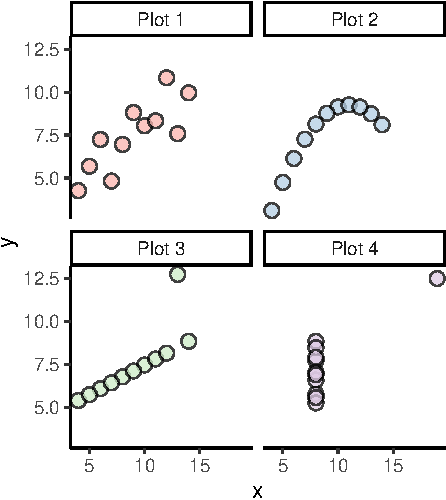
\includegraphics{confirmationreport_files/figure-pdf/fig-anscombe-1.pdf}

}

\caption{\label{fig-anscombe}The four scatter plots that make up the
anscombe quartet. Each x and y variable has the same mean, standard
deviation, and correlation}

\end{figure}

Utilising visualisation can give people a more complete understanding of
risks. Studies asking participants to sketch a distribution allowed them
to better compute statistics about that distribution and improve
predictions (Hullman et al. 2018; Goldstein and Rothschild 2014). While
there is some evidence that confidence provided in text form only are
less likely to be misinterpretated than grahics (Savelli and Joslyn
2013), text is insufficient to express more complicated aspects of a
distribution, such as mass. The confusion caused by visualisation could
also be due to a lack of expose, since Kay et al. (2016) found that
people exposed to the same uncertainty visualisation get better at
making judgements the more they are exposed to them. Additionally,
visualisation allows for interactive graphics that provide a more in
depth understanding of probability (Potter et al. 2009a; Ancker, Chan,
and Kukafka 2009) and infographics that make uncertainty more accessible
for people with poor numeracy skills (Ancker, Chan, and Kukafka 2009).

Despite these benefits, there is a reasonable amount of annecdotal and
survey evidence that we don't visualise uncertainty as often as we
should. Some economists suggest that visualisation authors are
responding to incentives that make it tempting to avoid visualising
uncertainty, even if those incentives are based more in perception than
reality (Manski 2020). A survey conducted by Hullman (2020) found that
majority of visualisation authors agreed that expressing uncertainty is
important and should be done more often than it currently is, some even
agreed that failing to do so is tantamount to fraud. Despite this, only
a quarter of respondents included uncertainty in 50\% or more of their
visualisations (Hullman 2020). Meaning participants were convinced that
visualising uncertainty is morally important but were able to provide
self sufficient reasoning that allows them to avoid doing it. The study
by Hullman (2020) found that the most common reasons authors don't
visualise uncertainty in practice despite knowing it's moral importance
are: not wanting to overwhelm the audience; an inability to calculate
the uncertainty; a lack of access to the uncertainty information; and
not wanting to make their data seem questionable (Hullman 2020).

If decision markers are not presented with the uncertainty about an
estimate the data analysts have, for all intents and purposes, made the
decision for the decision maker. Upon further interviews Hullman (2020)
found that authors believed uncertainty would overwhelm the audience and
make their data seem questionable because decision makers are unable to
understand uncertainty. This belief, while pervasive, is not true. While
some research suggests that laypeople cannot understand complicated
concepts in statistical thinking (such as trick questions on hypothesis
tests or the difference between Frequentist and Baysian thinking)
(Hoekstra et al. 2014; Bella et al. 2005) there is a large amount of
research suggesting that presenting uncertainty information improves
decision making, both experimentally (Joslyn and LeClerc 2012; Savelli
and Joslyn 2013; Kay et al. 2016; Fernandes et al. 2018) and in practice
(Al-Kassab et al. 2014). As a matter of fact, doing what many authors
currently do (providing only a deterministic outcome with no
uncertainty) causes decision makers to be \emph{less} decisive and have
completely unbounded expectations on an outcome (Savelli and Joslyn
2013). This reality cannot be avoided by providing secondary or
non-specific information such as explaining calculations (Joslyn and
LeClerc 2012), explaining the advantages of a recommendation (Joslyn and
LeClerc 2012), or expressing uncertainty in vague terms (Erev and Cohen
1990; Olson and Budescu 1997), all of which are undesirable for decision
makers and lead to measurably worse decisions (Joslyn and LeClerc 2012;
Erev and Cohen 1990; Olson and Budescu 1997). Expressing uncertainty
verbally additionally decreases the percieved reliability and
trustworthiness of the source (Bles et al. 2020). One of the most
popular depictions of uncertainty for decision making is a quantile
dotplot, shown in Figure~\ref{fig-quantdot}.

\begin{figure}

{\centering 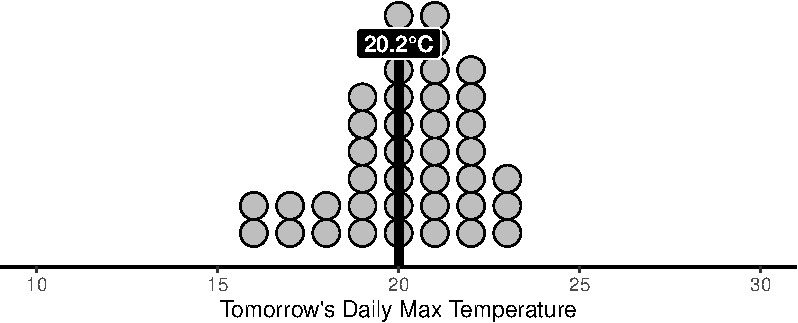
\includegraphics{confirmationreport_files/figure-pdf/fig-quantdot-1.pdf}

}

\caption{\label{fig-quantdot}A quantile dotplot is an uncertainty
visualisation that provides a discrete display of uncertainty to aid
decision making. This example plot provides an estimate for a daily
maximum temperature.}

\end{figure}

Not only does communicating uncertainty improve decisions but the
mistrust created by communicating certainty in uncertain situations can
be exploited. A 6-month survey of anti-mask groups on Facebook during to
COVID-19 pandemic showed that the anti-maskers thought carefully about
their grammer of graphics and made pursuasive visualisations using the
same data as pro-mask groups by exploiting information ignored by the
pro-maskers (Lee et al. 2021). It is understood that deceptive plots can
lead viewers to come to incorrect conclusions or significantly overstate
effects or risks (Pandey et al. 2015; L. Padilla et al. 2022) but these
incorrect takeaways cannot be mitigated with instructions in how to
correctly understand the plot (Boone, Gunalp, and Hegarty 2018). This
evidence indicates we are more likely than not to hurt our message when
we ignore uncertainty information and trying to raise the general
publics plot literacy is an insufficient strategy to curb conspiracy
theories and misguided scientific communication. In direct contrast to
this, displaying numerical estimates of uncertainty information has
shown to lead to greater trust in predicitions (Joslyn and LeClerc 2012;
Bles et al. 2020). While Han et al. (2009) found people have more worry
when presented with uncertainty reguarding health outcomes, this worry
is not a bad thing if the concern is warranted given the ambiguous
situation.

The disconnect between the research supporting uncertainty and the
consensus aganinst may not be entirely driven by a lack of understanding
of the literature. For example, at least one interviewee from the study
by Hullman (2020) claimed that expertise implies that the signal being
conveyed is significant, but also said they would omit uncertainty if it
obfuscated the message they were trying to convey (Hullman 2020). Other
authors who were capable of calculating and and representing uncertainty
well did not do it, and were unable to provide a self-satisfying reason
why (Hullman 2020). These conflicting motivations are acknowledged in
the paper itself where Hullman (2020) says:

\begin{quote}
``It is worth noting that many authors seemed confident in stating
rationales, as though they perceived them to be truths that do not
require examples to demonstrate. It is possible that rationales for
omission represent ingrained beliefs more than conclusions authors have
drawn from concrete experiences attempting to convey uncertainty''.
\end{quote}

An overwhelming consensus among visualisation authors seems to be that
uncertainty is secondary to estimations. There is a belief help by those
that work with data that the uncertainty associated with an estimate
(the noise) only exists to hide the estimate itself (the signal). From
this view, uncertainty is only seen as additional or hindering
information, therefore despite its alleged importance, when simplifying
a plot uncertainty the first thing to go. This belief is also reflected
in the development of new uncertainty visualisations. Often when trying
to visualise a high problem, uncertainty is relegated to unimportant
aesthetics in the plot, often of lower importance than the estimate
(Correll, Moritz, and Heer 2018; Lydia R. Lucchesi and Wikle 2017). This
is not uncommon with high dimensional data considering spatial temporal
data often Cases where uncertainty is not relegated to an undesirable
aesthetic instead incorporate interactivity to allow users to explore
the complicated space themselves (Potter et al. 2009b, 2009a). Even the
literature about uncertainty communication expresses an implicit belief
that it is of secondary importance to the estimates or context of the
data.

An adjacent issue is \emph{how much} uncertainty we should include when
trying to quantify our associated distribution. Obviously the correct
answer is somewhere between ``every possible outcome'' which would
result in an unbounded uncertainty and ``a simple confidence interval
based on a set of strict and unrealistic assumptions'' that would result
in an interval that is far too narrow. Unfortunately between those two
extremes the solution is largely a judgement decision which can
sometimes be overwhelming. This is why software that provides
\emph{some} uncertainty visualisation as a default, such as forecasts in
the \texttt{fable} package are useful (O'Hara-Wild, Hyndman, and Wang
2023). It prevents authors omitting uncertainty through inaction. There
is the possibility, however, that default uncertainty visualisations
facilitate the poor understanding of which conclusions are relevant to
the uncertainty visualised.

This issue is not helped by the fact that the term ``uncertainty'' lacks
a commonly accepted definition in the literature. Lipshitz and Strauss
(1997) even commented that ``there are almost as many definitions of
uncertainty as there are treatments of the subject'' . This mishmash of
terminology leads to a large body of work, all claiming to finding the
best visualisation or expression of of ``uncertainty'' but most don't
even seem to agree on what uncertainty is. The most encompassing
definition of uncertainty I have seen comes from Walker et al. (2003)
who define uncertainty as \textbf{``any deviation from the unachievable
ideal of completely deterministic knowledge of the relevant system''}.
This definition does not completely align with the distribution
conceptualisation I discussed earlier in this chapter, but the cases
where they diverge are rare and can still be handled by focusing on the
relevant information. More commonly, uncertainty is defined using a
taxonomy rather than a strict definition. There are a few of taxonomies
for uncertainty, but, just like the definition, most of them are a
subset of the one laid out by Walker et al. (2003).

Figure~\ref{fig-taxonomy} is an illustration of the taxonomy presented
by Walker et al. (2003). In this taxonomy, there are three things we
need to consider for each ``uncertainty'' we encounter through the
modelling process. First, consider the source of the uncertainty. Is
this uncertainty coming from inaccurate measurements or a poorly defined
model? This is the \emph{location} of the uncertainty. Second, consider
how well you can quantify this uncertainty. Do you know exactly how much
measurement error there is in each observation or are you not even aware
if there is or isn't measurement error? This is the \emph{level} of your
uncertainty, and it ranges from discrete to total ignorance. Finally,
consider how this uncertainty came into existence. Is it a result of a
naturally random process (epistemic) or is it due to imperfect
information and could be improved (aleatory). This is the \emph{nature}
of your uncertainty. Walker et al. (2003) then go on to describe mapping
our uncertainty in a 3D space that is defined by its location, level,
and nature, but I think the taxonomy is more easily understood as a
series of questions we need to consider when asking how much unertainty
we should express to our audience.

\begin{figure}

{\centering 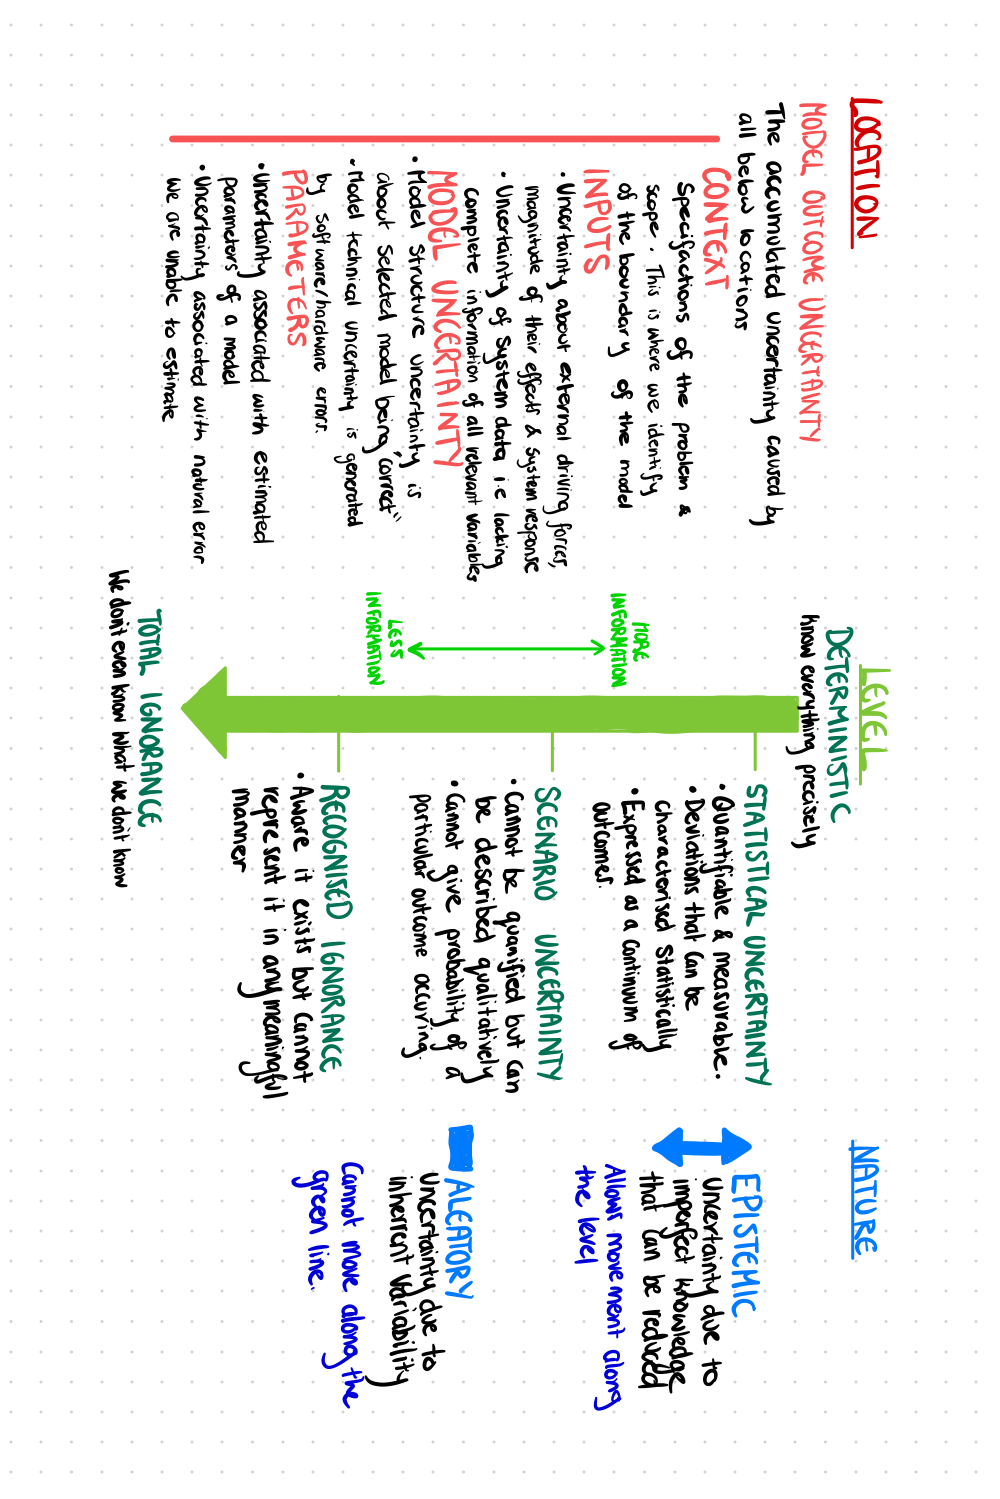
\includegraphics{taxonomyvis.jpeg}

}

\caption{\label{fig-taxonomy}Illustration of the taxonomy described in
Walker et al. (2003)}

\end{figure}

While information about the sources of our uncertainty and the type of
uncertainty may seem like an unimportant secondary step in uncertainty
visualisation, communicating these features of uncertainty helps
decision makers make more informed choices. L. M. K. Padilla et al.
(2021) found that low forecaster confidence or high model uncertainty
both contribute to more conservative judgements by decision makers.
Failling to communicate the nature of your uncertainty can result in
underestimation or overestimation of failure probabilities (Kiureghian
and Ditlevsen 2009). Additionally Gustafson and Rice (2019) found that
the framing of our uncertainty, (i.e.~informing the reading if the
uncertainty came from a lack of knowledge, approximations, unknown
unknowns, or disagreement among parties) does not have a significant
effect on the belief in the estimates, perceived credibility, or
behavioral intentions of the decision makers. This means communicating
secondary information about your uncertainty is unlikely to negatively
affect your communication and is important in understanding the scope of
your uncertainty.

The use of uncertainty in high dimensional environments is especially
important in energy data. Large models that incorporate spatial-temporal
data from many sources and systems are used to predict energy uses in
the short and long term. Understanding how to improve and make better
decisions in these models is imperative in both the daily operation of
the energy sector as well as the transition from fossile fuels to clean
energy. Therefore the energy sector is an incredibly relevant
application of research in uncertainty visualisation techniques.

\newpage{}

\hypertarget{thesis-overview}{%
\section{Thesis Overview}\label{thesis-overview}}

The overarching theme of my thesis is a change in the way we understand
uncertainty visualisations, specifically in the case of communication.
This work will be divided into three chapters.

\hypertarget{chapter-1-a-new-theoretical-framework}{%
\subsection{Chapter 1: A new theoretical
framework}\label{chapter-1-a-new-theoretical-framework}}

Chapter 1 discuss the current state of the research surrounding
uncertainty visualisation and describe two fundamental mistakes in the
way researchers conceptualise uncertainty visualisations. The first
mistake is in the role of distributions in the visualisation framework,
where irrelevant distributions are used to answer questions and relevant
distributions are ignored. These distribution issues are mistakenly
reported as visualisation issues in the literature, ignoring a
fundamental statistical problem in the way we visualise uncertainty. The
second mistake is a belief that uncertainty visualisation will improve
while uncertainty is seen as of low importance. I highlight how a lot of
research in imporoving uncertainty visualisation reflects the belief
that uncertainty is inherrently unimportant. I suggest that there is no
overarching best uncertainty visualisation, but rather uncertainty
visualisations should depend on a motivating question. Finally I provide
a framework for visualising uncertainty that mitigates these issues by
ensuring the visualisation author decides on the motivations and of
their graphic, can correctly identify the relevant distribution and the
aspects of the distribution that are needed for their motivation; and
correctly assigns priority to these apects by using the correct
aesthetics.

\hypertarget{chapter-2-applications-of-the-framework}{%
\subsection{Chapter 2: Applications of the
framework}\label{chapter-2-applications-of-the-framework}}

Chapter 2 applies this framework and investigates its practical
usefullness through experiemnts and discussions with AEMO. The purpose
of data visualisation is insight, but due to time limits or other
constraints, most visualisation studies use multiple benchmark tests as
a substitute for measuring the complicated phenomena of insight (North
2006). Unfortunately the validity of these results hinge on the large
insights we gain from graphics being the sum total of these small
incremental insights which may not always be true (North 2006).
Specifically in uncertainty visualisation, there is a focus on
performance and accuracy based measures that assume more predictabe
behaviour from people than what research on human decision making
suggests. The work in Chapter 2 should avoid these common pitfalls that
arrise from experimental plot evaluations by working closely with people
at AEMO. Our partners at AEMO will be able to provide detailled and open
ended descriptions of the beenfits and struggles of our uncertainty
visualisation techniques. This allow us to directly see the improvements
(or lack thereof) in insight due to the suggested framework.

\hypertarget{chapter-3-translation}{%
\subsection{Chapter 3: Translation}\label{chapter-3-translation}}

Chapter 3 will be a translation of chapter 1 and 2 into an R package.
This will make this research more accessible and allow others to easily
implement this visualisation framework in their own work.

\newpage{}

\hypertarget{chapter-1-a-new-theortical-framework}{%
\section{Chapter 1: A new theortical
framework}\label{chapter-1-a-new-theortical-framework}}

\hypertarget{the-current-landscape-of-visualisation-experiments}{%
\subsection{The current landscape of visualisation
experiments}\label{the-current-landscape-of-visualisation-experiments}}

Current research in visualising uncertainty seems to have a focus on
designing new options for visualising uncertainty for specific types of
data. Typical papers comparing visualisation methods seem to fit into
one or both of the follow categories:

\begin{enumerate}
\def\labelenumi{\arabic{enumi})}
\item
  a paper that suggests or compares uncertainty visualisations that
  depict a single distribution.
\item
  a paper that suggests or compares uncertainty visualisations for a
  specific type of data
\end{enumerate}

Generally the goal seems to be to increase the number of options we have
in our ``visualisation bag'' so that we always have a plot at the ready
if we want to visualise uncertainty. These new plots also tend to focus
on a catch all plot that is ``best for making decision'' or ``best for
visualising spatial uncertainty''. Data visualisation is commonly
utilised as a tool in data exploration, so it is not uncommon for a data
analyst to make a plot with only a vague goal and use it to pull out a
large number of adjacent observations. For example, a data analyst might
make a scatter plot to find out the relationship between two variables,
but in doing do also finds out that one variable has discrete outcomes
over a range of values. It is common knowledge that any single plot
cannot reveal all information about a data set, all plot types obfuscate
and uncover different types of information, however this aspect of
plotting becomes more apparent in uncertainty visualisation. Often when
discussing ``uncertainty'' information, we expect readers to be able to
draw information from a plot that was not estimated, prioritised, or
visualised. Communicating uncertainty can be boilled down into two
simple steps, first we need to quantify the uncertainty, and second, we
need to communicate it (Webster 2003). The two issues I have noticed in
uncertainty visualisation literature each come from one of these steps.
The first issue is failing to identify the correct distribution
(quantifying) and the second is failling to select a visualisation that
highlights the important aspects of the distribution (communicating).
These issues run deep in the literature, but they are easiest to
understand with an example that I will repeatedly return to as we
develop this idea.

\hypertarget{part-1-distribution}{%
\subsection{Part 1: Distribution}\label{part-1-distribution}}

\hypertarget{example-comparing-hops-error-bars-and-violin-plots}{%
\subsubsection{Example: Comparing HOPs, error bars, and violin
plots}\label{example-comparing-hops-error-bars-and-violin-plots}}

The issues that are rampant in the uncertainty visualisation literature
are easily seen if we zoom in on one example. The study done by Hullman,
Resnick, and Adar (2015) is a great illustration in the importance of
having a clear motivation when you design a graphic. It is important to
keep in mind that while I am primarily discussing one paper to
illustrate a point, the issues I am brining to light are the standard in
the uncertainty visualisation literature. This paper is no outlier.

The study by Hullman, Resnick, and Adar (2015) asked participants to
provide some numerical properties of a distribution using a hypothetical
outcome plot (HOPs), an error bar plot or violin plot. Participants were
given questions relating to individual and multiple distributions. When
shown a single distribution participants were asked about the mean of
the distribution, the probability of an outcome being above some
threshold (indicated on the plot with a red dot), or the probability of
an outcome being between two given values. When shown two distributions
the participants were asked ``How often is measurement of solute B
larger than the measurement of solute A?'', and when shown three
distributions ``How often is measurement of solute B larger than the
measurement of solute A and solute C?''. Figure~\ref{fig-examples} shows
an example error bar plot and violin plot for the two distribution case.
There was also a high and low variance case for every plot and question
combination. The study decided which technique was better using absolute
error between the subjects response and the true value. They specified
that the error bars are not confidence intervals as they represent the
true underlying distribution, not the sampling distribution of the mean.
They found that the HOPs reliably outperformed the violin and error bar
plots for all the two and three distribution questions, but were no
better than the violin or error bar plot in the other univariate cases
(and in some cases worse).

\begin{figure}

\begin{minipage}[t]{0.50\linewidth}

{\centering 

\raisebox{-\height}{

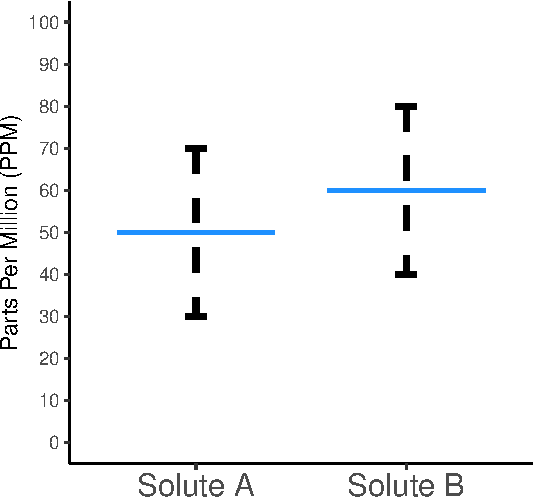
\includegraphics{confirmationreport_files/figure-pdf/fig-examples-1.pdf}

}

}

\subcaption{\label{fig-examples-1}Error bar plot}
\end{minipage}%
%
\begin{minipage}[t]{0.50\linewidth}

{\centering 

\raisebox{-\height}{

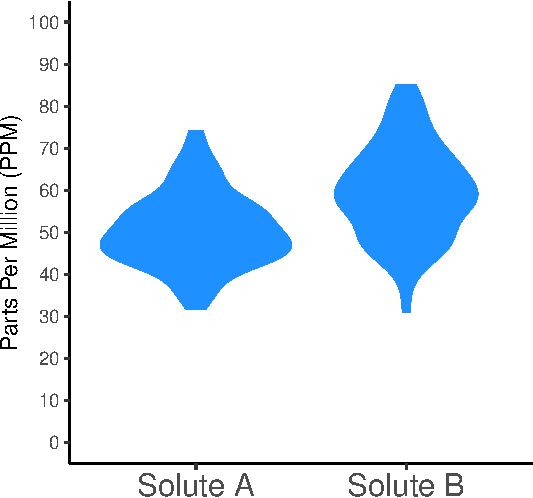
\includegraphics{confirmationreport_files/figure-pdf/fig-examples-2.pdf}

}

}

\subcaption{\label{fig-examples-2}Violin plot}
\end{minipage}%

\caption{\label{fig-examples}An example of the plots shown in the two
variable tasks given in (Hullman, Resnick, and Adar 2015). The example
question provided with this plot was `In what percentage of vials is
there more of solute B than A (Probability(B \textgreater{} A)?'}

\end{figure}

My first issue with the plots in Hullman, Resnick, and Adar (2015) study
is that the violin plot and error bars are visualising a different
distribution to the HOPs plot. The error bar plot and the violin plot in
Figure~\ref{fig-examples} visualise the marginal distributions of
solutions A and B and provides no information on the joint distribution.
The HOPs plot is similar to a slope graph except instead of connecting
the outcomes from A and B with a line, they are connected through frames
of an animation. The HOPs, just like a slope graph, depicts a
relationship between two varibles, i.e.~the \emph{joint} distribution.
This key feature can be used to improve upon the HOPs and direct our
attention to the distribution that is even more useful for answering
this question.

Two alternative graphics that could be used to answer the question ``In
what percentage of vials is there more of solute B than A (Probability(B
\textgreater{} A)?'' are provided in Figure~\ref{fig-alternatives}. The
scatter plot depicts the joint distribution of the two solutions and
uses colour to highlight the Bernoulli distribution that is more closely
aligned with the question. The stacked bar exclusively visualises the
Bernouli distribution that describes the event \(B>A\) and ignores the
joint distribution highlighted by the scatter plot. Through this process
of moving from the marginal distributions, to the joint distribution to
the bernouli distributionm we moved the information needed to answer the
question ``What is \(P(B>A)\)?'' from something you needed to calculate
in your head (when looking at the error bar plots) to something you can
\textbf{see} in the bar chart. While this process is illuminating, it is
important to avoid whittling down the problem \textbf{too} much.
Providing a categorical decision alone is somewhat useless, it is
important to ballance advice with uncertainty estimates as a ballance of
the two results in the most accurate decisions (Joslyn and LeClerc
2012).

\begin{figure}

\begin{minipage}[t]{0.50\linewidth}

{\centering 

\raisebox{-\height}{

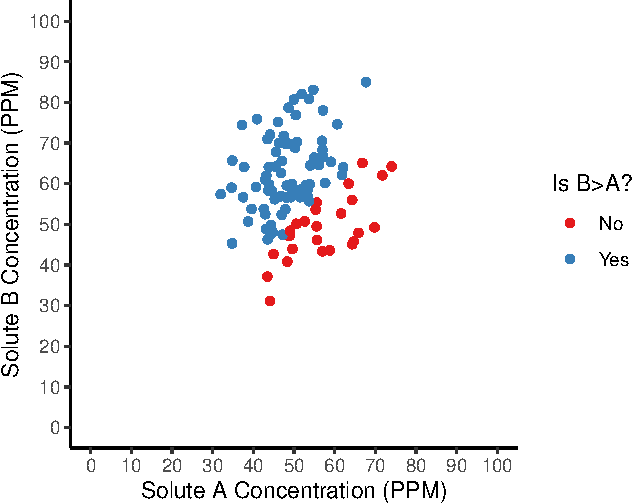
\includegraphics{confirmationreport_files/figure-pdf/fig-alternatives-1.pdf}

}

}

\subcaption{\label{fig-alternatives-1}Scatter Plot}
\end{minipage}%
%
\begin{minipage}[t]{0.50\linewidth}

{\centering 

\raisebox{-\height}{

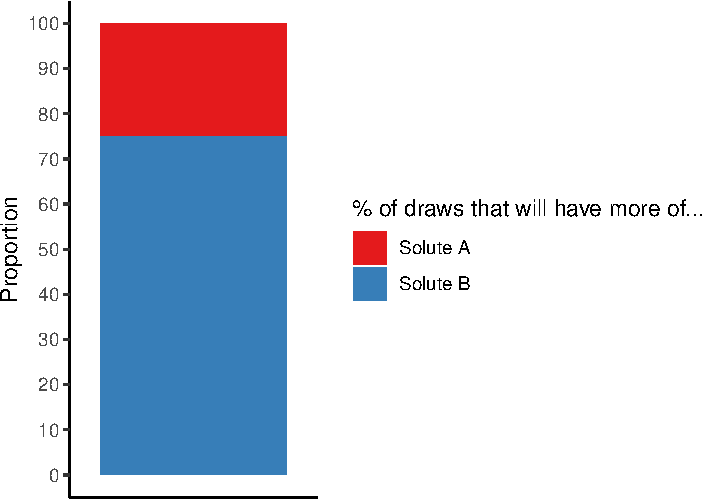
\includegraphics{confirmationreport_files/figure-pdf/fig-alternatives-2.pdf}

}

}

\subcaption{\label{fig-alternatives-2}Stacked Bar Chart}
\end{minipage}%

\caption{\label{fig-alternatives}Two plots that could be used as
alternatives to answer to question `In what percentage of vials is there
more of solute B than A (Probability(B \textgreater{} A)?'. The scatter
plot in (a) focuses on the relationship between the concentration of
solute A and solute B, while the stacked bar chart in (b) highlights the
frequency with which each solute is greater than the other.}

\end{figure}

\hypertarget{theory-selecting-the-correct-distribution}{%
\subsubsection{Theory: Selecting the correct
distribution}\label{theory-selecting-the-correct-distribution}}

In order to fairly compare two uncertainty visualisations, they need to
provide the same information. This is rarely done in plots comparing
distribution visualisations. The important distinction between the
distribution displayed and the distribution required to answer a
question is often ignored in our discussions good or bad uncertainty
visualizations. This means that studies identifying some graphics as
better than others may only do so because the two plots displayed
different distributions. Figure~\ref{fig-distdraw} illustrates how we
think about distributions when performing statsitical tests compared to
when we create visualisations. When we compute statistics or perform a
hypothesis test, we typically put a lot of thought into what the correct
distribution is for our question, however, when we perform visualisation
we typically plot a collection of normal marginal distributions and
ignore the actual distribution required. This extends to our perception
of visualisation in general as most of the visualisation we consider to
be for ``distributions'' are actually just tools for visualising
marginal distributions.

\begin{figure}

{\centering 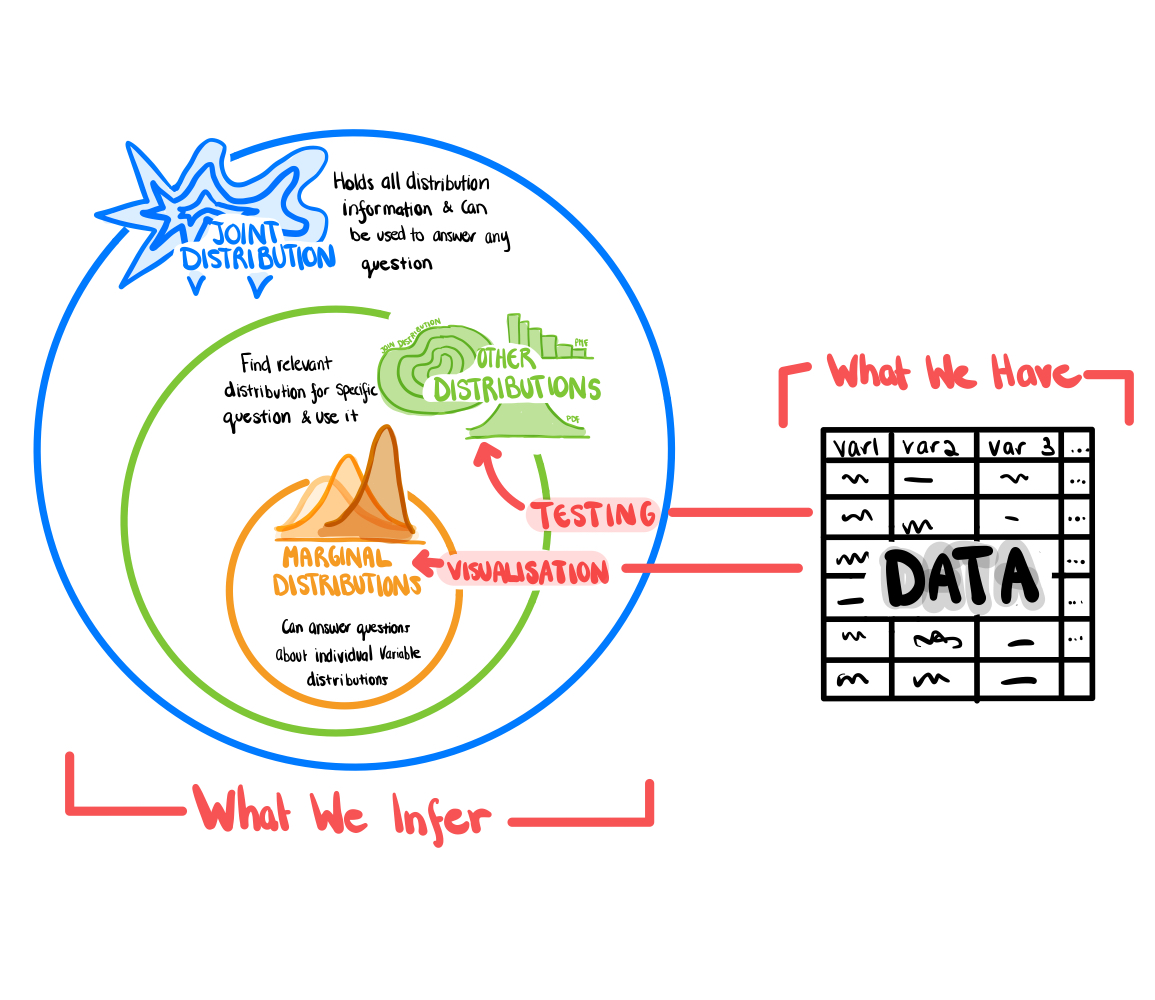
\includegraphics{incorrectdistributions.jpeg}

}

\caption{\label{fig-distdraw}Illustration depicting the difference
between the distributions we use for testing vs the visualisation we
visualise}

\end{figure}

An example that might be more familiar to the average statistician is
something I like to refer to as ``the error bar problem''. If you have
ever looked at two overlapping error bars and said ``oh these variables
are not statistically significantly different'' you have used error bars
incorrectly. While it is true that error bars that do not overlap
implies statistical significance, overlapping error bars do not imply
the converse in true. The same is true for a lot of the other ad-hoc
statistical tests we use error bars for. A study done by Bella et al.
(2005) asked participants to adjust two error bars until the means were
``just'' statistically significantly different, and most people adjusted
the error bars until they were just touching. In the case of independent
confidence intervals that just touch, the p-value of the associated
two-tailled t-test is about 0.006 (Schenker and Gentleman 2001). Bella
et al. (2005) also found that few people could incorporate changing
information about independence that arrises from repeated measure design
and most participants were ignorant to the fact that error bars are used
for both confidence intervals and standard error bars, two wildly
different indicators of precision.

This is a classic example of expecting readers to draw conclusions about
a distribution that was not visualised. Error bars typically represent
the 95\% confidence interval of a sampling distribution, most commonly
the significant values of a t-distribution. This means that each error
bar provides the range of significant values through the two end points,
and a vague indicator of variance with the length of the bar, \emph{of
each variable independently}. What an error bar does \textbf{not} depict
is the t-distribution associated with a difference of two means, the
equivalent statistical test we utilise error bars for. The visualisation
itself is not the problem, trying to draw conclusions that requires
information that was not visualised is.

The papers that go on to cite these misunderstandings about error bars
discuss the work as though the problems are caused by error bars
themselves. They suggest that error bars should be avoided as a
visualisation tool, ignoring the fact that these fundamental
misunderstandings in uncertainty will likely follow other visual
encodings of t-distributions. Maybe some visual aspect of error bars
encourages these extrapolations, but the HOPs example I drew on at the
start of this chapter illustrates that this problem of expecting people
to answer questions that are not directly related to the visualised
distribution is larger than questions about significance.

This view of understanding uncertainty visualizations opens up a new gap
in the literature. For example, if we accept that visualizing a
collection of t-distributions is not a substitute for a collection of
F-tests or paired t-tests, how \emph{should} we visualise uncertainty if
we want to draw those conclusions? Rather than shutting down the
discussion on the usefulness of visualisation, I beleive it opens it and
highlights areas of improvement in our current work.

\hypertarget{part-2-features}{%
\subsection{Part 2: Features}\label{part-2-features}}

\hypertarget{example-more}{%
\subsubsection{Example: more}\label{example-more}}

Let us return to the study done by Hullman, Resnick, and Adar (2015).
Not only is the distribution depicted in the visualisation different,
but the features of the distribution depicted are also different. In
discussing the concept of a ``best'' visualisation, we rarely discuss
which \emph{features} of the distribution are being displayed in the
graphic. The way we currently look at visualisation would classify the
error bar plot and the violin plot as visualisations of a
``distribution'', the scatter plot is a visualisation of a
``relationship'' while the bar plot is a visualisation of ``amounts''
(Wilke (2019)), but this categorisation hides a lot of important details
about drawing information from a graph. In this example the violin plot
and the scatter plot both showed that each solution had an independent
marginal normal distribution, the error bar (although technically a plot
for visualising distributions) gives no concept of mass and would not
give you the ability to identify even a simple distribution. Not only is
it important to select a distribution that is appropriate for our
question, it is also important to \emph{show} the aspect of that
distribution that holds the relevant information. The example asked
about the \emph{frequency} of a particular outcome which translates to
visualising the \emph{outcomes} of the joint distribution \textbf{or}
the \emph{parameter} of the Bernoulli distribution since these are the
aspects of each distribution that hold the information we are looking
for. If we visualised features of the distribution that don't hold the
information we are looking for, the information is difficult to
assertain and is more likely to be found through potentially faulty
heuristics.

Figure~\ref{fig-bad} depicts two graphics that have the of the same
distributions as those in Figure~\ref{fig-alternatives}, but each plot
visualises an aspect of the distribution that is less relevant to the
question. The 2D error bar plot (or circle?) highlights the mean and the
values that are within the 95\% confidence range. Since none of the
parameters of the joint distribution are directly related to the
question at hand, visualising the mean and significance instead of the
outcomes made it harder to answer ``What is \(P(B>A)\)?''. Since the
parameter of the Bernouli distribution \emph{is} directly related to the
question, visualising outcomes makes it harder to answer the question.

\begin{figure}

\begin{minipage}[t]{0.50\linewidth}

{\centering 

\raisebox{-\height}{

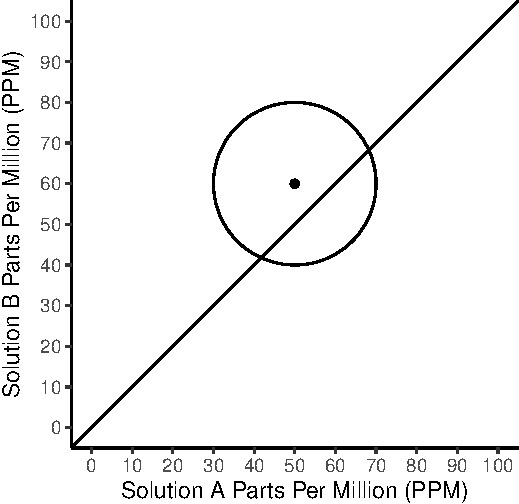
\includegraphics{confirmationreport_files/figure-pdf/fig-bad-1.pdf}

}

}

\subcaption{\label{fig-bad-1}Error cirlce. The point in the middle
represents the mean and the circle represents the area 95\% of values
will fall into.}
\end{minipage}%
%
\begin{minipage}[t]{0.50\linewidth}

{\centering 

\raisebox{-\height}{

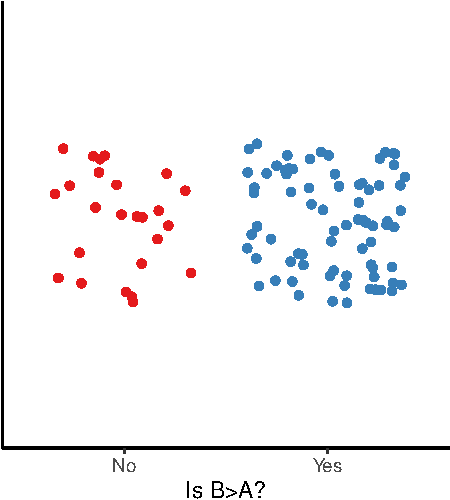
\includegraphics{confirmationreport_files/figure-pdf/fig-bad-2.pdf}

}

}

\subcaption{\label{fig-bad-2}A scatter plot depicting the samples of the
bernouli distribution}
\end{minipage}%

\caption{\label{fig-bad}Two plots that are not useful in answering the
question `In what percentage of vials is there more of solute B than A
(Probability(B \textgreater{} A)?'. While the distributions visualised
are correct, we have visualised the incorrect feature of the repsective
distributions. Plot (a) visualises mean and significance thresholds of
for values (b) the.}

\end{figure}

Not only does visualising the incorrect distribution that highlights
incorrect features related to a question make it difficult to answer
correctly, it might also completely disorientate the viewer. In the
discussion of the study Hullman, Resnick, and Adar (2015) notes:
\textgreater{} ``In light of the common usage of error bars for
presenting multiple independent distributions, it is noteworthy how
poorly subjects using these representations performed on tasks asking
them to assess how reliably a draw from one variable was larger than the
other\ldots Many subjects reported values less than 50\%, which are not
plausible given that the mean of B was larger than the mean of A.''

\hypertarget{theory-the-four-features-of-a-distribution}{%
\subsubsection{Theory: the four features of a
distribution}\label{theory-the-four-features-of-a-distribution}}

Different features of a distribution have different questions they are
mode adept adept at answering. The apsect of a distribution that are
typically depicted in graphics can be organised into four key features.
Figure~\ref{fig-features} depicts these four features along with an
example of how they are typically depicted in graphics. Each of these
four features have a set of questions they are better equip to answer.
The four features are:

\begin{enumerate}
\def\labelenumi{\arabic{enumi})}
\item
  \textbf{Mass} describes the PMF/PDF or CMF/CDF of the functions.
  Depictions of mass can inform us of the mode, likely or impossible
  values, and whether or not we have an identifiable distribution.
\item
  \textbf{Samples} are a set of actual or simulated outcomes of a
  distribution. Our data falls into this category as it can be seen as
  an outcome of some ``underlying'' distribution. Outcomes can also be
  simulated through techniques such as bootstrapping or random sampling.
  Outcomes are useful to answer questions about frequency, however since
  outcomes have a connection to mass (depending on the structure of the
  graphic, a mass plot may just be a smoothed plot of a visualisation of
  a sample) they can sometimes be used to answer the same questions.
\item
  \textbf{Parameters} are the statistics that are related to our
  distribution. They can be the sufficient statistics of the
  distribution, such as the mean, variance, minimum and maximum, or they
  can be other statistics such as the or correlation, median and mode.
  Visualising a specific parameter of our distribution typically gives
  us freedom because it allows us to express any aspect of a plot in
  terms of a single value. Unfortunately this flexibility means that the
  set of question questions a parameter plot can answer are limited.
  Questions about the mean, median, maximum, minimum, correlation,
  values of significance, etc would usually need multiple plots to
  answer.
\item
  \textbf{Exchangability} illustrates whether or not a elements in a
  sequence of random variables from this distribution can be swapped.
  Rather than answering questions about exchangability, it is something
  we typically want to highlight in our data. Exchangability is often
  expressed by having features touch in a graphic. A time series
  inechangability is expressed using a line plot, spatial data's
  inechangability is expressed using a map and the exchangability of
  randomly sampled data is often expressed using points. Exchangability
  is adjacent to continuity because visually connected features in a
  graphic are also used to express discretised outcomes of a continuous
  process (such as a ridgeline plot).
\end{enumerate}

\begin{figure}

{\centering 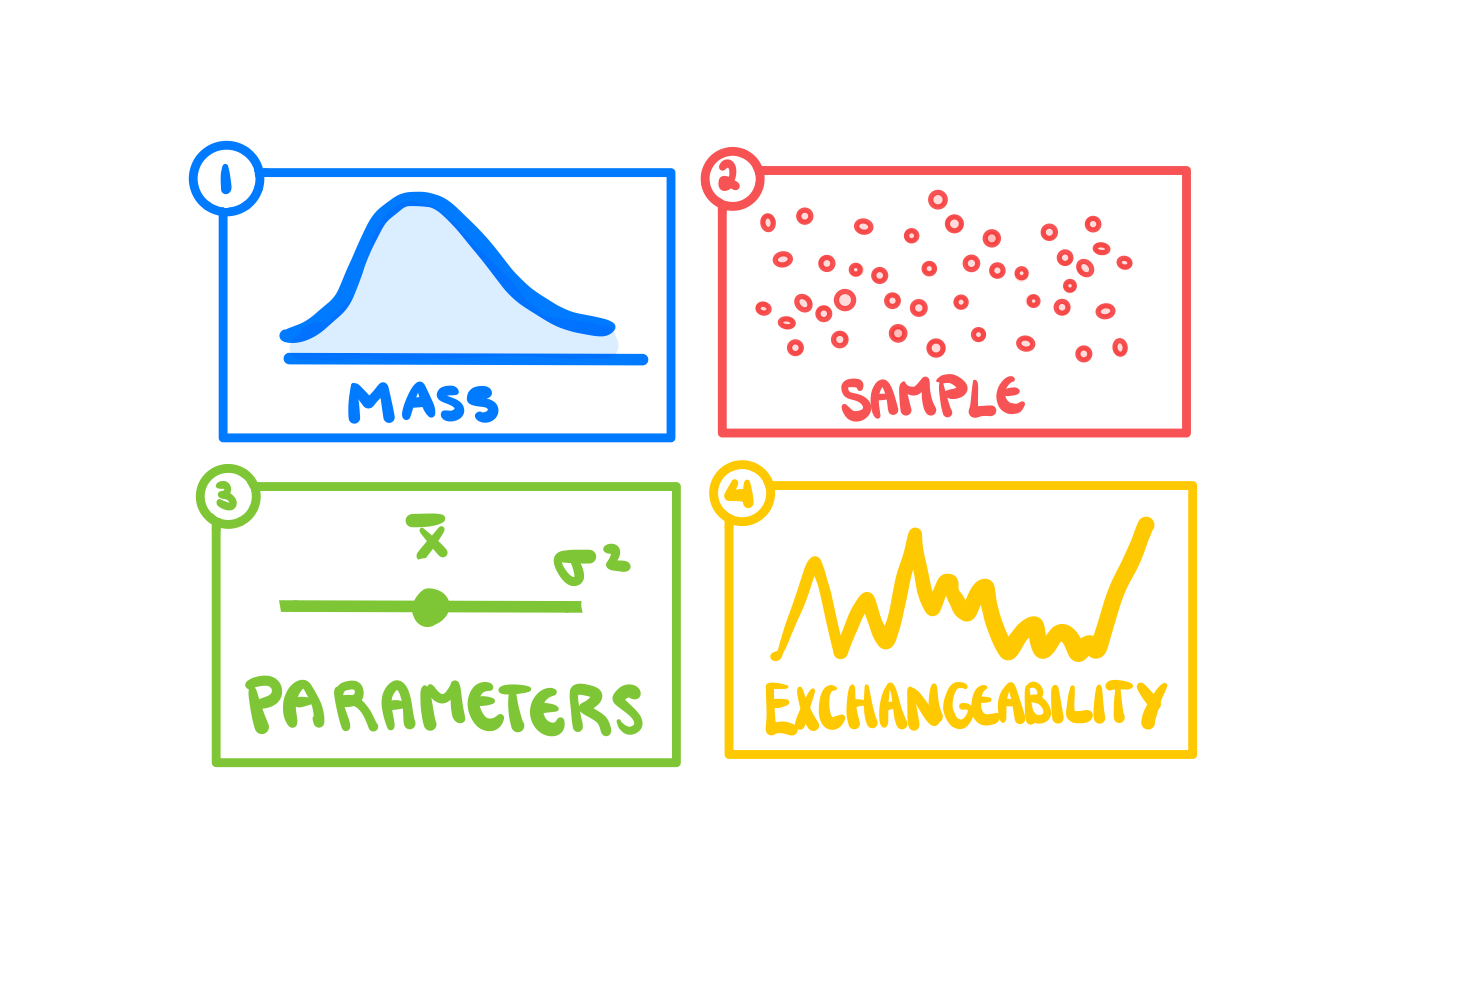
\includegraphics{distfeatures.jpeg}

}

\caption{\label{fig-features}The four main features of a distribution
graphics are typically used to represent}

\end{figure}

This is not an exhaustive list of every possible feature of a
distribution, but rather the four most commonly visualised aspects of a
distribution. Additionally, these features are not entirely distinct,
particular visualsiations of parameters or samples may also double as a
depiction of mass. Therefore, a graphic that is designed to depict one
feature of a distribution may depict multiple features of multiple
distributions. It also compares multiple ways of showing distribution to
see which has more power.

\hypertarget{part-3-hierarchy}{%
\subsection{Part 3: Hierarchy}\label{part-3-hierarchy}}

\hypertarget{example-looking-to-spatial-uncertainty}{%
\subsubsection{Example: Looking to spatial
uncertainty}\label{example-looking-to-spatial-uncertainty}}

This chapter so far has focused on the first way in which we talk about
``visualising uncertainty'' which is to depict some aspect of a
distribution, however this does not cover the case of visualising
uncertainty to express the impreciseness of estimates. Often our goal in
visualisation is not to perform a statistical test or to make a decision
based on a single estimate, but to identify some underlying structure in
our data or make a decision based on a large number of connected
systems. Visualising estimates and the uncertainty associated with those
estimates separately can lead to the uncertainty being ignored (Moritz
et al. 2017). This is typically the case when we try and visualise
spatial uncertainty.

Trying to depict the uncertainty of an estimates with a spatial aspect
is incredibly difficult. Even displaying an estimate in a spatial
context can have problems. Improvements in spatial plots typically focus
on ways to map a distribution that is dependent on something other than
land size while still depicting the inexchangability and location that
is relevant to spatial data. A common complaint about choropleth maps is
that they depict the estimated parameter as a function of land size
instead of location, even if land size is irrelevant to the estimate
(such as in the case of voting). Visualisations that correct for this,
such as hex maps, do so by colouring and plotting hexagonal tiles that
each represent a portion of the dependent location (Kobakian and Cook,
n.d.). This means an irrelevant feature, such as land size is not
depicted as important in the map. Trying to highlight the uncertainty
associated with these estimates makes the process even more difficult.

There are four proposed methods of visualising spatial uncertainty that
can be made with the \texttt{Vizumap} R package (Lydia R. Lucchesi,
Kuhnert, and Wikle 2021). These four plots each present uncertainty with
varying degrees of success and failure.

The two visualiations that do a reasonably good job of expressing error
are the bivariate map and the pixel map. Figure~\ref{fig-spatialuncert1}
depicts these two types of visualisation. Plot (a) depicts a bivariate
map which uses a bivariate colour palette which is created by blending
two single hue colour palettes. One colour represents the variable of
interest while the other represents uncertainty. There are two immediate
problems with this method. First of all, uncertainty is being mapped
with hue and saturation. Figure~\ref{fig-huesatcol} illustrates the
differences between hue, saturation, and value when looking at a colour
palette. Maceachren et al. (2012) found hue and saturation to be two of
the worst aesthetics to map to uncertainty as they don't have an
intuitive connection to uncertainty and so participants were worse.
Value does have a natural connection to uncertainty (lighter values
equate to higher uncertainty and darker values equate to more certainty)
so it is a much more appropriate choice. While the \texttt{Vizumap} data
does depict areas of light and darkenss, they are largely irrlevant to
the uncertainty measure causing our heuristics to lead us to the
incorrect conclusions. The Value-Suppressing Uncertainty Palettes (VSUP)
shown in Figure~\ref{fig-vsup} maps estimates to the hue and uncertainty
to the value thereby creating a more intuitive plot (Correll, Moritz,
and Heer 2018 ). Additionally, at high levels of uncertainty VSUP only
has one output colour, which explicitly prevents any decoding of one
output colour without enforcing a binary encoding of significance
(Correll, Moritz, and Heer 2018). Unfortunately VSUP are not easy to
combine with packages like \texttt{Vizumap} which leaves it still
somewhat difficult to express this encoding in practice, however the
combination of a bivariate map with VSUP has shown to improve decisions
in the face of uncertainty (Correll, Moritz, and Heer 2018). Plot (b)
from Figure~\ref{fig-spatialuncert1} depicts a pixel map. Pixel maps are
similar to HOPs plots since they present a sample of possible values for
the estimate, rather than a single value and an uncertainty
visualsiation. Some depictions of a pixel map are quite intuitive, such
as those shown in Bauer and Rose (2015), however these cases link
``uncertainty'' to sparseness rather than a wide array of potential
outcomes. Currently the effectivness of a pixel map is yet to be shown
in any experients, and it may turn out to be a poor encoding of
uncertainty information. Mapping a distribution of colours to numerical
values is currently required to extract actual values from the plot
which is a relatively difficult mental task Therefore the pixel map
might be more effective if values were written explicitly on top of the
pixels. The pixel map is also quite computationally expensive and hard
to interpret when the relevant geographical areas are small relative to
a large map, so it is likely best used on simpler smaller geographical
areas.

\begin{figure}

{\centering 

\begin{figure}

{\centering 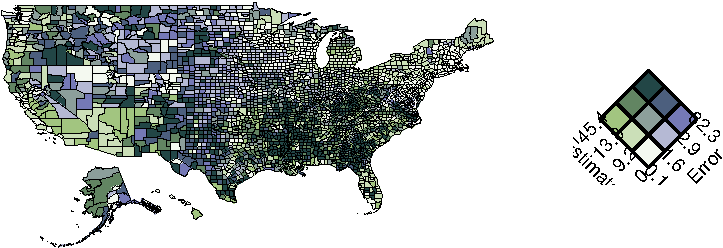
\includegraphics{confirmationreport_files/figure-pdf/fig-spatialuncert1-1.pdf}

}

\caption{Bivariate map}

\end{figure}

\begin{figure}

{\centering 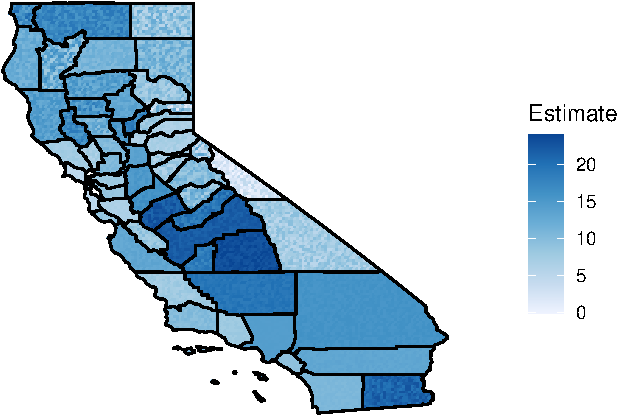
\includegraphics{confirmationreport_files/figure-pdf/fig-spatialuncert1-2.pdf}

}

\caption{Pixel map}

\end{figure}

}

\caption{\label{fig-spatialuncert1}The two more inventive visualisations
of spatial uncertainty that can be made using the \texttt{Vizumap}
package. These are the example visualisations of the bivariate and pixel
map that are provided in the package vingette.}

\end{figure}

\begin{figure}

{\centering 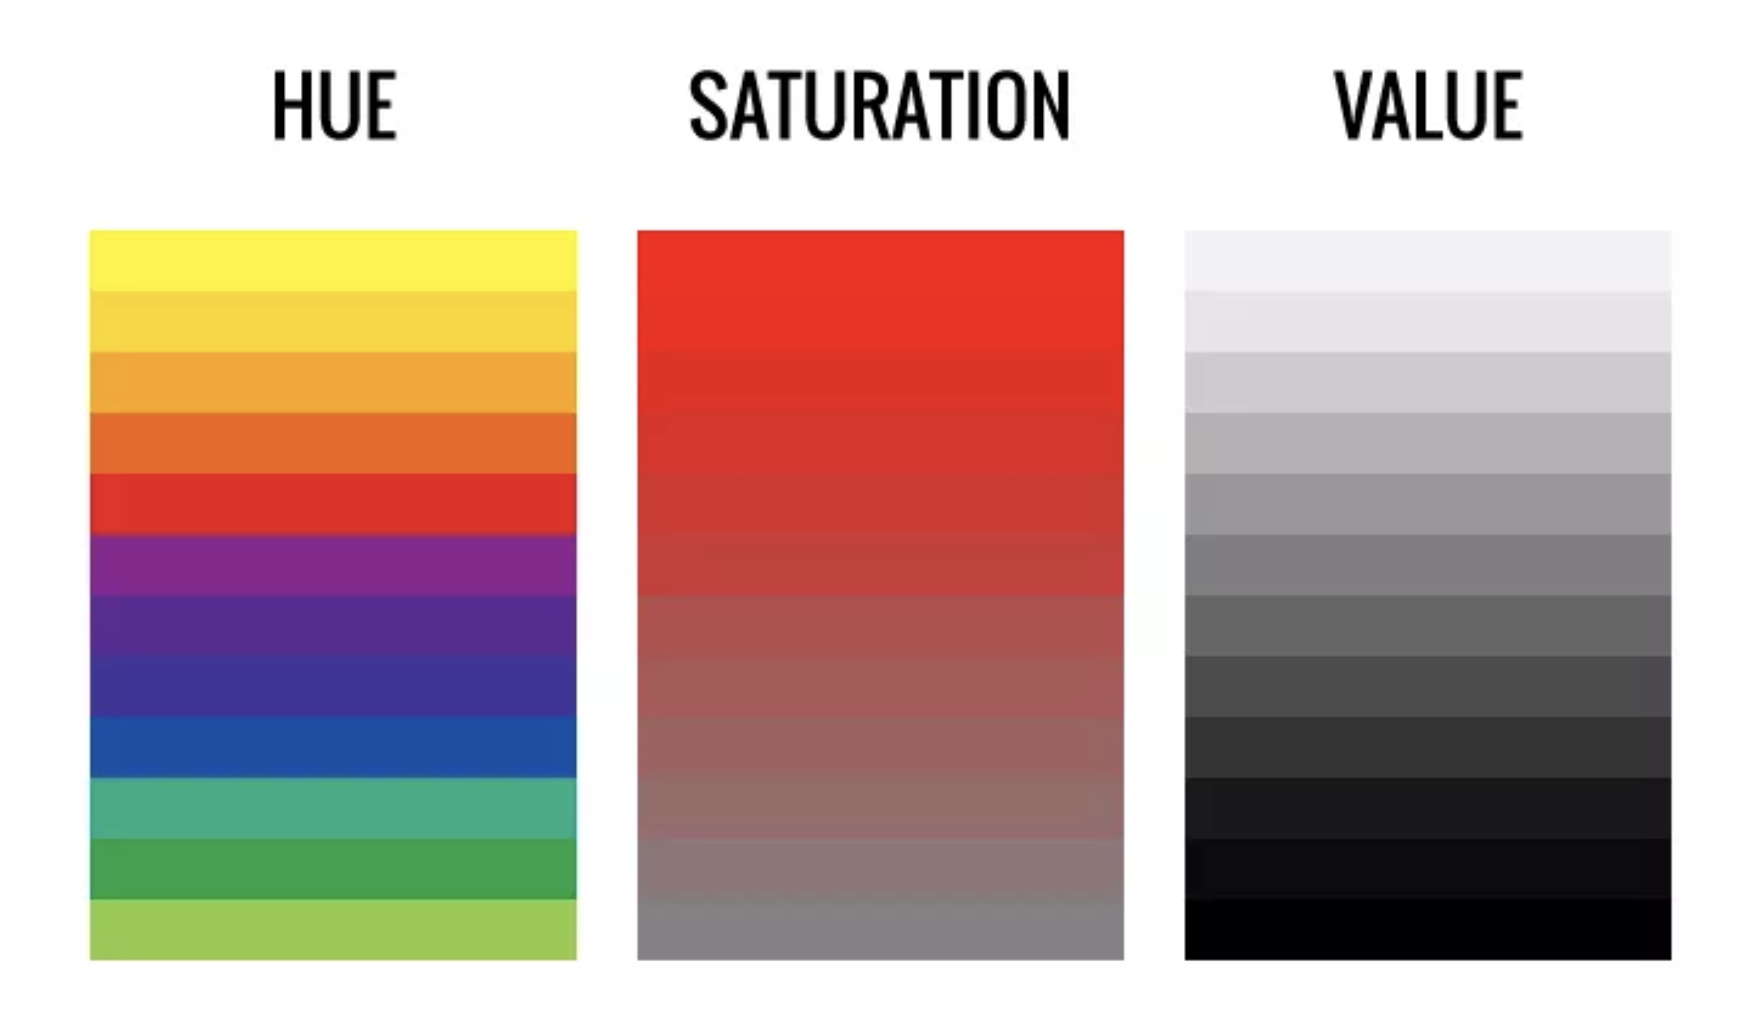
\includegraphics{huesatval.png}

}

\caption{\label{fig-huesatcol}Visual depiction of hue, saturation and
value of a colour palette from Makhdoomi (2021)}

\end{figure}

\begin{figure}

{\centering 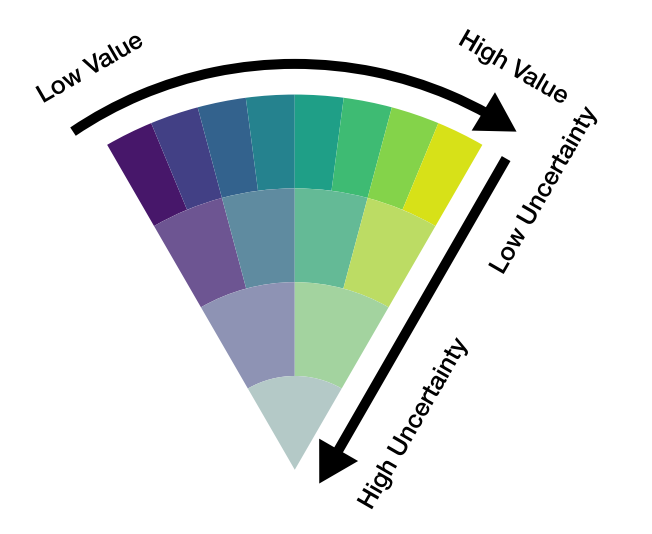
\includegraphics{vsup.png}

}

\caption{\label{fig-vsup}An example of a Value-Suppressing Uncertainty
Palette with axis aids}

\end{figure}

Figure~\ref{fig-spatialuncert2} depicts the two plots that are either
inappropriate for depicting spatial error, or are functionally the same
as maps that already exist. Plot (c) is a glyph map that uses colour of
a glyph to express the estimate and the rotation of the glyph to express
uncertainty. Orientation has no intuitive link to uncertaitny and should
be avoided at all costs (Maceachren et al. 2012). This plot also makes
it easier to ignore the uncertainty all together since it is mapped to a
feature that is different to the estimate. Plot (d) is a exceedance
probability map that shows the probability of the estimate being over a
certain value. This plot was developed specifically for decision making
relative to a single value in mind, and can be considered a
visualisation of a single parameter (Kuhnert et al. 2018). An exceedance
probability map map is actually very similar to a chloropleth map, but
instead of expressing an estimate, it shows a probability. Therefore
this plot is only able to express probability through a change in
information rather than an improvement in visualisation techniques.

\begin{figure}

{\centering 

\begin{verbatim}
  0%  25%  50%  75% 100% 
 0.0  8.1 11.3 15.1 45.4 
\end{verbatim}

\begin{figure}

{\centering 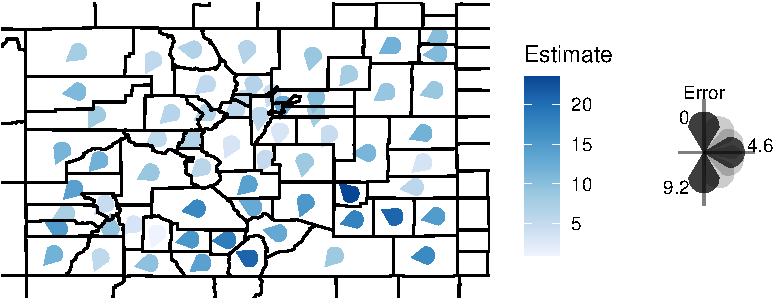
\includegraphics{confirmationreport_files/figure-pdf/fig-spatialuncert2-1.pdf}

}

\caption{Glyph map}

\end{figure}

\begin{figure}

{\centering 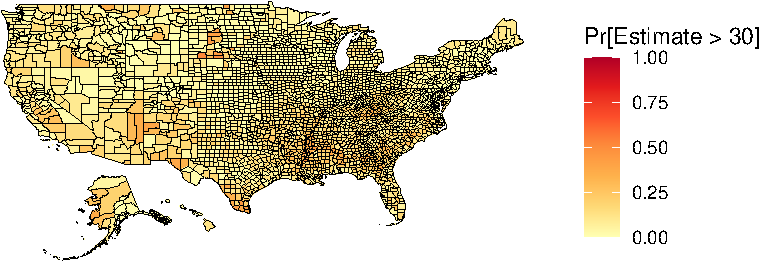
\includegraphics{confirmationreport_files/figure-pdf/fig-spatialuncert2-2.pdf}

}

\caption{Exceedance probability map}

\end{figure}

}

\caption{\label{fig-spatialuncert2}The two visualisations of spatial
uncertainty that can be made using the \texttt{Vizumap} package that are
less impressive. The glyph map is already used in high dimensional data
and rotation is a poor mapping for error. An exceedance probability map
is useful for uncertainty visualisaitons, but it is functionally the
same as a chloropleth map.}

\end{figure}

The four plots depicted in Figure~\ref{fig-spatialuncert1} and
Figure~\ref{fig-spatialuncert2} are not the be all end and all of
visualisation of spatial uncertainty. They are a suggested solution for
a particular case of uncertainty visualisation, when we want to
highlight the certainty or uncertainty associated with a particular
estimate. They may not even always work in that case depending on the
complexity of the underlying distribution. The plots that can be
expressed using \texttt{Visumap} sets a particular order of importance
to the information we are conveying (typically geographical information
\textgreater{} estimate \textgreater{} sample uncertainty) and maps that
information to aesthetics that are of relative importance in the plot.

\hypertarget{theory-mapping-the-features-to-the-appropriate-hierarchy}{%
\subsubsection{Theory: Mapping the features to the appropriate
hierarchy}\label{theory-mapping-the-features-to-the-appropriate-hierarchy}}

The methods I discussed in parts 1 and 2 of this chapter and the method
I discussed in the starting example of this section are not as distinct
as I am making them out to be. We can think of this new problem using
the framing I have established so far in this chapter. This question
boils down to ``how do I visualise the sampling distriubtions of large
number of estimates and also visualise some features of a larger
distribution that THOSE estimates came from''. When there are many
features of the data that are competing for our interest, we often don't
have as much flexibility in how we choose to visualise uncertainty.
Frequently we abandon complicated features of our distributions, such as
mass, to make way for for complicated features of the data such as
spatial dependence. Obviously every possible piece of information you
might want to depict in a plot cannot be extrated with maximum
efficiency, so we need to establish some kind of hierarchy.

A hierarchy of elementary perception tasks is not a new idea in
visualisation. Cleveland and McGill (1984) found a natural ordering of
10 elementary perception tasks in term of how accurately participants
could extract information that was mapped to that feature. The hierarchy
established was: 1) Position along a common scale 2) Positions along
nonaligned scales 3) Length, direction (slope), angle 4) Area 5) Volume,
curvature 6) Shading, color saturation While Cleveland and McGill (1984)
notes that these tasks are not exhaustive nor mutually exclusive, and
accuracy is not the only metric that should decide if a graphic is
worthwhile, this hierarchy does provide a useful rule of thumb in
understanding the importance of information we are illustrating in a
graph. Therefore, not only should we consider what information we are
depicting in our graph, we should also consider the implicit information
hierarchy our graphic displays. It is one thing to have information in a
plot, it is another for this information to be displayed in a way that
allows for the information to be \emph{efficiently} extracted. Previous
discussions on hierarchy focused on mapping specific variables to
elementary tasks, but I am combining the idea with the concept of
relevant features and asking what features of each distribution do you
think are important.

Additionally, just because information is in a graphic, that does not
mean it will be ``seen''. The phenomena of inattentional blindness shows
that there is no perception without attention and it is powerful enough
that participants can fail to be aware of random objects appearing on a
screen or a gorilla walking through a basketball game {[}Simons and
Chabris (1999); mack2003inattentional{]}. Therefore if information is
mapped to graphical elements that are so low on hierarchy they can be
ignored, they might as well not be there at all. Therefore the people
who don't plot uncertainty because they think its unimportant and the
people who relegate uncertainty to the lowest ranking aesthetic on the
list are both saying the same thing, ``I think the uncertainty is
unimportant''. Including uncertainty is worth very little if no
attention is left to see it. That is not to say we cannot put a
\emph{large} amount of information in a graphic, glyph maps can be used
to depict the multi-dimensional information in spatial-temporal data,
but we still need to decide what information is important. Differenct
scales can be used depending on whether you want to identify trends in
global variance or local variance (Wickham et al. 2012), and smaller
details are almost impossible to convey. No matter how much information
we try and put in a plot, there will always be only a hanful of key take
aways.

Not only should we considered the hierarchy in the information we
depict, but we also need to consider the heuristics that connect some
pieces of information to specific elementary tasks. For example Hofmann
et al. (2012) showed that polar co-ordinates are more effective than
catesian co-ordinates when considering data that depicts directions
which have a naturally polar interpretation. Uncertainty is naturally
mapped to Fuziness, location, colour value best, then arrangement, size
and transparency are an OK second choice, while saturation, hue,
orientation and shape are unacceptable and have no intuitive connection
to variance (Maceachren et al. 2012). No only do the graphical elements
we map our features to matter, but the direction matters too. Graphical
elements that are more fuzzy (fuziness), further from center (location),
lighter (colour value), poorly arranged (arrangement), smaller (size),
more transparent (transparency) are percieved to be more uncertain
(Maceachren et al. 2012). This idea also extends to interval estimation,
since gradient expressions are best for questions about probaility, but
ambiguation is best for start and end time estimation (Gschwandtnei et
al. 2016). Heuristics can work against us just as much as they can work
for us. The sine illusion can cause the confidence interval of a
smoothed sine curve to seem wider at the peaks than the troughs, causing
us to underestimate uncertainty associated with changing values
(Vanderplas and Hofmann 2015).

There is an assumption in visualsiation that we need to show enough
information to solve a task while avoiding irrelevant distracting
information (Kosslyn 2006). While including additional features can
increase the accuracies of some conclusions, it can also bias or
discount others. Including means estimates on depictions of mass can
cause people to discount the uncertainty information and use the
difference between means as a proxy (Kale, Kay, and Hullman 2021).
Tomasetti and Cook (2015) found that a scatter plot is better than a
line plot if you want to convey the correlation between two time series.
Unfortunately we cannot be sure if this was influenced by swapping the
conditional distribution for the joint distribution on the high priority
position axis, or by dropping the visualisation of the time series
exchangeability feature. Figure~\ref{fig-timescatter} depicts four
different visualisations of the same time series data. Each plot depicts
a different combination of distribution (joint or conditional on time)
and exchangability (the inechangability is either depicted with
connected values or ignored with points).

\begin{figure}

\begin{minipage}[t]{0.50\linewidth}

{\centering 

\raisebox{-\height}{

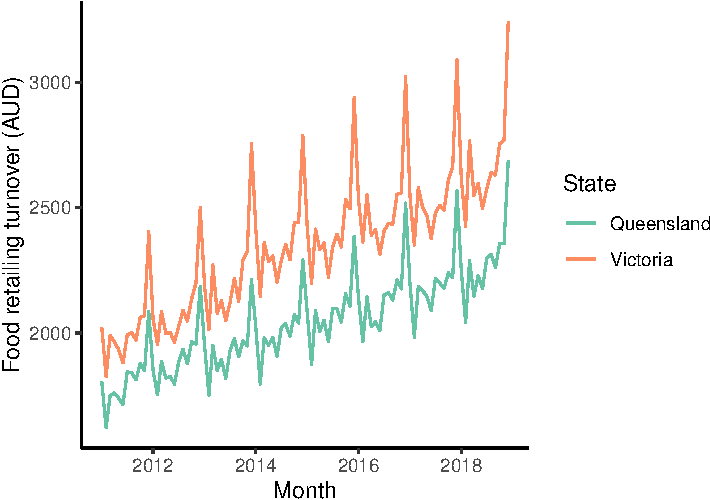
\includegraphics{confirmationreport_files/figure-pdf/fig-timescatter-1.pdf}

}

}

\subcaption{\label{fig-timescatter-1}Conditional distribution on time
with inexchangability}
\end{minipage}%
%
\begin{minipage}[t]{0.50\linewidth}

{\centering 

\raisebox{-\height}{

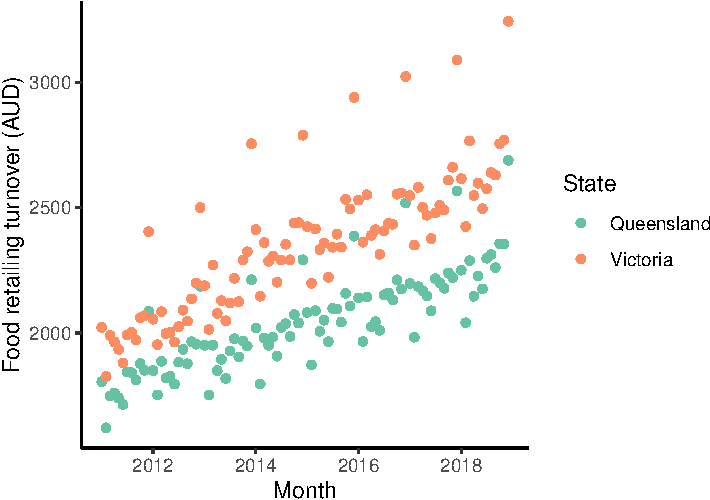
\includegraphics{confirmationreport_files/figure-pdf/fig-timescatter-2.pdf}

}

}

\subcaption{\label{fig-timescatter-2}Conditional distribution on time}
\end{minipage}%
\newline
\begin{minipage}[t]{0.50\linewidth}

{\centering 

\raisebox{-\height}{

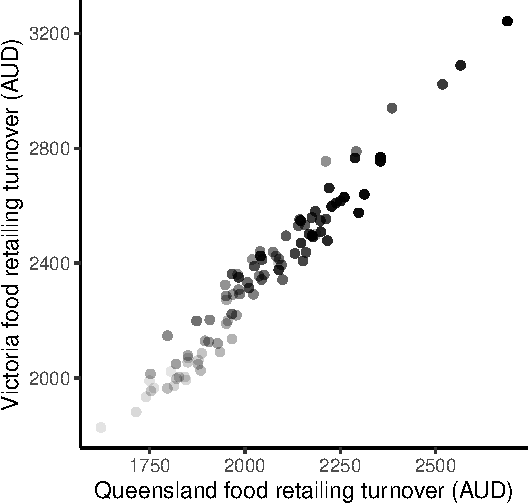
\includegraphics{confirmationreport_files/figure-pdf/fig-timescatter-3.pdf}

}

}

\subcaption{\label{fig-timescatter-3}Joint distribution of series}
\end{minipage}%
%
\begin{minipage}[t]{0.50\linewidth}

{\centering 

\raisebox{-\height}{

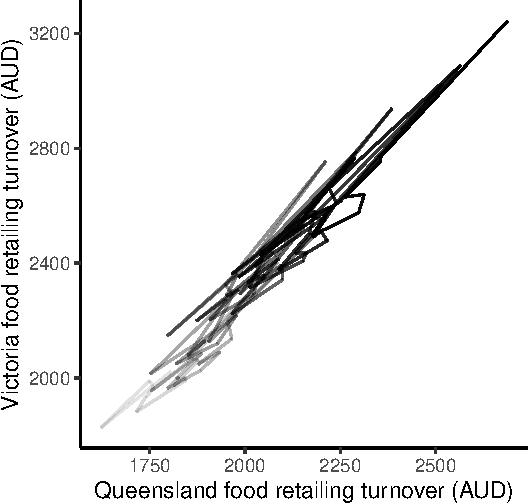
\includegraphics{confirmationreport_files/figure-pdf/fig-timescatter-4.pdf}

}

}

\subcaption{\label{fig-timescatter-4}Joint distribution of series with
inexchangability}
\end{minipage}%

\caption{\label{fig-timescatter}Four figures to illustrate the impact of
changing the priority of the distribution displayed and presence of
exchangeability . Time is depicted with opacity in plots (c) and (d) to
maintain the same information. More recent dates are darker. Could you
order these four plots by how well they convey correlation?}

\end{figure}

With this in mind lets assess the hierarchy established in the figures
of Figure~\ref{fig-spatialuncert1} and Figure~\ref{fig-spatialuncert2}.
Despite being against the categorisation of ``uncertainty'',
``estimate'', and ``data'' I will use it here because it is how it is
referred to in the literature. Plot (a) in set the estimate and
uncertainty at the same level of importance, plot (b) visualised the
uncertainty over the estimate. Roation does not exist in the hierarchy
(direction refers to identifying slopes and angles are for vectors
starting at the same origin) and I found it easy to ignore, therefore
plot (c) sets ``uncertainty'' is at a lower level than the estimate.
Plot (d) displays a parameter related to both the estimate and its
uncertainty. All four plots place spatial information at the highest
level of importance. If the only thing you want from your plot is a
sense of estimates with respect to their position in space, these plots
are fine, but what if there is a feature of your distribution that is of
higher importance than the order/inexchangeability of your data? Playing
around with this hierarchy and asking if the same features of our
distribution are being conveyed can lead to some interesting plots, such
as those depicted in Figure~\ref{fig-timescatter}.

What should become apparent comparing these plots is that there is a
constant trade off between information relevant to the our question and
secondary information that provides context. By always assuming features
such as the spatial context are always the most important apsect of a
plot, we kneecap research and don't consider the wide array of ways we
can express complicated concepts such as inexchangability and perception
heavy information such as location.

\hypertarget{why-this-taxonomy}{%
\subsection{Why this taxonomy?}\label{why-this-taxonomy}}

You may wonder what the point of this alternative taxonomy is. There
many other visualisation taxonomies that may feel more natural than the
one I present here. For example Grewal, Goodwin, and Dwyer (2021)
categorized uncertainty visualizations based on discreteness of the
distribution (a sub feature of mass) and the domain expertise (something
I don't cover). Hofmann et al. (2012) classified uncertainty
distributions by the level of data summation, a measure that was
adjacent to the number of data points used to construct the graphic, but
the plots made were also all depictions of different distributions
features. Wilke (2019) organised all graphics, not just uncertainty
visualisations, into 7 categories (with large overlaps). These groups
were amounts, distributions, proportions, x-y relationships, geospatial
data, and uncertainty. There is also evidence that the way we express
the mass of a distribution is important even though it is something my
taxonomy does not cover. There is a reasonable amount of evidence that
cumulative displays or discrete displays (such as a quantile dot-plots
or histograms) are the best ways to express mass for decision making and
probability estimates {[}Fernandes et al. (2018); Hofmann et al. (2012);
Kay2016; Hullman et al. (2018){]}.

Despite these alternatives I still believe this taxonomy is filling a
gap in the literature for two reasons. First of all this taxonomy allows
us to properly evaluate the results of any visualisation paper (not just
uncertainty specific ones). By reading the questions asked of
participants, identifying the relevant distribution and feature, and
then identifying which plot maps that feature to the highest ranking
elementary perception task, you can often guess the conclusion of a
visualisation paper with a high degree of accuracy. There are a handful
of questions the taxonomy does not resolve (e.g.~comparing a different
marginal densities or comparing catesian vs polar co-ordinates), but a
large number of experiments that compare two plots that supply different
information become self evident. The second benefit of the taxonomy is
it provides a simple set of questions any visualisation author can ask
themselves to identiy if their plot conveys the message they are trying
to communicate. Every plot conveys information and if you want your
audience to answer a question about the plot, it needs to convey a
\emph{sufficient} amount of relevant information for the audience to
draw their conclusions. This taxonomy allows not only allows us to
understand what may be wrong with some visualisations, but it also
provides suggestions to improve a visualisation once you understand the
motivation.

Unfortunately visualisation papers that properly consider the underlying
distributional information depicted in a plot are rare, and papers that
don't conflate issues created by an incorrect distribution, incorrect
features, or poor use of aesthetics even more so.

\newpage{}

\hypertarget{timeline}{%
\section{Timeline}\label{timeline}}

A timetable for completing the thesis and a statement of progress to
date (make sure to match everything to apsects of the thesis) - (done)
Literature review (have made progress in this year) have picked up main
parts of the infoviz community - changed topic once got new scholarship
(check off to say completed) - can pencil in energy aspect now (met with
them earlier in the year) - have a need for this work - next meeting in
June (and have regular meetings monthly over the next year and hopefully
build up applications) - Have idea of when I think I will have a
finished piece of work (literature review) - Content for each of the
pieces should be mapped out - ASC later in year (submitted an abstract
for a poster) - getting design of experiment clear and question we want
to answer clear can go round and round (good idea to have something
simple to test) - dont have time for something too complicated in phd
need to have it in small managable pieces - ASC december 2023 - apsect
of literature review + results from preliminary experiemnt - IEEE VIS
(June 22 2023 poster abstract) - Conference October 2023 (present aspect
of literature review) - The Rstudio conference (posit conference) - hard
to get a spot (worth applying for) - Aim for something international in
a year (or in last year) - Also could do UseR! 2024 (or 2025) \& talk
about some of the software developed (technical output) - Could have an
energy specific one (various applied energy) - IEEE VIS (march 31st
paper due in 2025) - Conference October 2025 (Vienna) - Thesis due
December 2025

\newpage{}

\hypertarget{bibliography}{%
\section*{Bibliography}\label{bibliography}}
\addcontentsline{toc}{section}{Bibliography}

\hypertarget{refs}{}
\begin{CSLReferences}{1}{0}
\leavevmode\vadjust pre{\hypertarget{ref-Al-Kassab2014}{}}%
Al-Kassab, Jasser, Zied M Ouertani, Giovanni Schiuma, and Andy Neely.
2014. {``{Information visualization to support management decisions}.''}
\emph{International Journal of Information Technology \& Decision
Making} 13 (2): 407--28.
\url{https://doi.org/10.1142/S0219622014500497}.

\leavevmode\vadjust pre{\hypertarget{ref-Ancker2009}{}}%
Ancker, Jessica S., Connie Chan, and Rita Kukafka. 2009. {``{Interactive
graphics for expressing health risks: Development and qualitative
evaluation}.''} \emph{Journal of Health Communication} 14 (5): 461--75.
\url{https://doi.org/10.1080/10810730903032960}.

\leavevmode\vadjust pre{\hypertarget{ref-anscombe}{}}%
Anscombe, F. J. 1973. {``Graphs in Statistical Analysis.''} \emph{The
American Statistician} 27 (1): 17--21.
\url{https://www.tandfonline.com/doi/abs/10.1080/00031305.1973.10478966}.

\leavevmode\vadjust pre{\hypertarget{ref-Bauer2015}{}}%
Bauer, Jennifer R., and Kelly Rose. 2015. {``{Variable Grid Method: An
Intuitive Approach for Simultaneously Quantifying and Visualizing
Spatial Data and Uncertainty}.''} \emph{Transactions in GIS} 19 (3):
377--97. \url{https://doi.org/10.1111/tgis.12158}.

\leavevmode\vadjust pre{\hypertarget{ref-Bella2005}{}}%
Bella, Sarah, Fiona Fidler, Jennifer Williams, and Geoff Cumming. 2005.
{``{Researchers misunderstand confidence intervals and standard error
bars}.''} \emph{Psychological Methods} 10 (4): 389--96.
\url{https://doi.org/10.1037/1082-989X.10.4.389}.

\leavevmode\vadjust pre{\hypertarget{ref-VanderBles2020}{}}%
Bles, Anne Marthe van der, Sander van der Linden, Alexandra L. J.
Freeman, and David J. Spiegelhalter. 2020. {``{The effects of
communicating uncertainty on public trust in facts and numbers}.''}
\emph{Proceedings of the National Academy of Sciences of the United
States of America} 117 (14): 7672--83.
\url{https://doi.org/10.1073/pnas.1913678117}.

\leavevmode\vadjust pre{\hypertarget{ref-Boone2018}{}}%
Boone, Alexander P., Peri Gunalp, and Mary Hegarty. 2018. {``{Explicit
versus actionable knowledge: The influence of explaining graphical
conventions on interpretation of hurricane forecast visualizations}.''}
\emph{Journal of Experimental Psychology: Applied} 24 (3): 275--95.
\url{https://doi.org/10.1037/xap0000166}.

\leavevmode\vadjust pre{\hypertarget{ref-Cleveland1984}{}}%
Cleveland, William S., and Robert McGill. 1984. {``{Graphical
perception: Theory, experimentation, and application to the development
of graphical methods}.''} \emph{Journal of the American Statistical
Association} 79 (387): 531--54.
\url{https://doi.org/10.1080/01621459.1984.10478080}.

\leavevmode\vadjust pre{\hypertarget{ref-Correll2018}{}}%
Correll, Michael, Dominik Moritz, and Jeffrey Heer. 2018.
{``{Value-suppressing uncertainty Palettes}.''} \emph{Conference on
Human Factors in Computing Systems - Proceedings} 2018-April: 1--11.
\url{https://doi.org/10.1145/3173574.3174216}.

\leavevmode\vadjust pre{\hypertarget{ref-Erev_1990}{}}%
Erev, Ido, and Brent L. Cohen. 1990. {``Verbal Versus Numerical
Probabilities: Efficiency, Biases, and the Preference Paradox☆.''}
\emph{Organizational Behavior and Human Decision Processes}.
\url{https://doi.org/10.1016/0749-5978(90)90002-q}.

\leavevmode\vadjust pre{\hypertarget{ref-Fernandes2018}{}}%
Fernandes, Michael, Logan Walls, Sean Munson, Jessica Hullman, and
Matthew Kay. 2018. {``{Uncertainty displays using quantile dotplots or
CDFs improve transit decision-making}.''} \emph{Conference on Human
Factors in Computing Systems - Proceedings} 2018-April: 1--12.
\url{https://doi.org/10.1145/3173574.3173718}.

\leavevmode\vadjust pre{\hypertarget{ref-Goldstein2014}{}}%
Goldstein, Daniel G., and David Rothschild. 2014. {``{Lay understanding
of probability distributions}.''} \emph{Judgment and Decision Making} 9
(1): 1--14.

\leavevmode\vadjust pre{\hypertarget{ref-Grewal2021}{}}%
Grewal, Yashvir, Sarah Goodwin, and Tim Dwyer. 2021. {``{Visualising
Temporal Uncertainty: A Taxonomy and Call for Systematic Evaluation}.''}
\emph{IEEE Pacific Visualization Symposium} 2021-April (April): 41--45.
\url{https://doi.org/10.1109/PACIFICVIS52677.2021.00013}.

\leavevmode\vadjust pre{\hypertarget{ref-Gschwandtnei2016}{}}%
Gschwandtnei, Theresia, Markus Bögl, Paolo Federico, and Silvia Miksch.
2016. {``{Visual Encodings of Temporal Uncertainty: A Comparative User
Study}.''} \emph{IEEE Transactions on Visualization and Computer
Graphics} 22 (1): 539--48.
\url{https://doi.org/10.1109/TVCG.2015.2467752}.

\leavevmode\vadjust pre{\hypertarget{ref-Gustafson2019}{}}%
Gustafson, Abel, and Ronald E. Rice. 2019. {``{The Effects of
Uncertainty Frames in Three Science Communication Topics}.''}
\emph{Science Communication} 41 (6): 679--706.
\url{https://doi.org/10.1177/1075547019870811}.

\leavevmode\vadjust pre{\hypertarget{ref-Han2009}{}}%
Han, Paul K. J., William M. P. Klein, Thomas C. Lehman, Holly Massett,
Simon C. Lee, and Andrew N. Freedman. 2009. {``{Laypersons' responses to
the communication of uncertainty regarding cancer risk estimates}.''}
\emph{Medical Decision Making} 29 (3): 391--403.
\url{https://doi.org/10.1177/0272989X08327396}.

\leavevmode\vadjust pre{\hypertarget{ref-Hoekstra2014}{}}%
Hoekstra, Rink, Richard D. Morey, Jeffrey N. Rouder, and Eric Jan
Wagenmakers. 2014. {``{Robust misinterpretation of confidence
intervals}.''} \emph{Psychonomic Bulletin and Review} 21 (5): 1157--64.
\url{https://doi.org/10.3758/s13423-013-0572-3}.

\leavevmode\vadjust pre{\hypertarget{ref-Hofmann2012}{}}%
Hofmann, Heike, Lendie Follett, Mahbubul Majumder, and Dianne Cook.
2012. {``{Graphical Tests for Power Comparison of Competing Designs}.''}
\url{http://www.public.iastate.edu/}.

\leavevmode\vadjust pre{\hypertarget{ref-Hullman2020a}{}}%
Hullman, Jessica. 2020. {``{Why Authors Don't Visualize Uncertainty}.''}
\emph{IEEE Transactions on Visualization and Computer Graphics} 26 (1):
130--39. \url{https://doi.org/10.1109/TVCG.2019.2934287}.

\leavevmode\vadjust pre{\hypertarget{ref-Hullman2018}{}}%
Hullman, Jessica, Matthew Kay, Yea Seul Kim, and Samana Shrestha. 2018.
{``{Imagining Replications: Graphical Prediction Discrete Visualizations
Improve Recall Estimation of Effect Uncertainty}.''} \emph{IEEE
Transactions on Visualization and Computer Graphics} 24 (1): 446--56.
\url{https://doi.org/10.1109/TVCG.2017.2743898}.

\leavevmode\vadjust pre{\hypertarget{ref-Hullman2015}{}}%
Hullman, Jessica, Paul Resnick, and Eytan Adar. 2015. {``{Hypothetical
outcome plots outperform error bars and violin plots for inferences
about reliability of variable ordering}.''} \emph{PLoS ONE} 10 (11).
\url{https://doi.org/10.1371/journal.pone.0142444}.

\leavevmode\vadjust pre{\hypertarget{ref-Joslyn2012}{}}%
Joslyn, Susan L., and Jared E. LeClerc. 2012. {``{Uncertainty forecasts
improve weather-related decisions and attenuate the effects of forecast
error}.''} \emph{Journal of Experimental Psychology: Applied} 18 (1):
126--40. \url{https://doi.org/10.1037/a0025185}.

\leavevmode\vadjust pre{\hypertarget{ref-Kale2021}{}}%
Kale, Alex, Matthew Kay, and Jessica Hullman. 2021. {``{Visual reasoning
strategies for effect size judgments and decisions}.''} \emph{IEEE
Transactions on Visualization and Computer Graphics} 27 (2): 272--82.
\url{https://doi.org/10.1109/TVCG.2020.3030335}.

\leavevmode\vadjust pre{\hypertarget{ref-Kay2016}{}}%
Kay, Matthew, Tara Kola, Jessica R. Hullman, and Sean A. Munson. 2016.
{``{When (ish) is my bus? User-centered visualizations of uncertainty in
everyday, mobile predictive systems}.''} \emph{Conference on Human
Factors in Computing Systems - Proceedings}, 5092--5103.
\url{https://doi.org/10.1145/2858036.2858558}.

\leavevmode\vadjust pre{\hypertarget{ref-Kiureghian2009}{}}%
Kiureghian, Armen Der, and Ove Ditlevsen. 2009. {``{Aleatory or
epistemic? Does it matter?}''} \emph{Structural Safety} 31 (2): 105--12.
\url{https://doi.org/10.1016/j.strusafe.2008.06.020}.

\leavevmode\vadjust pre{\hypertarget{ref-Kobakian}{}}%
Kobakian, Stephanie, and Dianne Cook. n.d. {``{Comparing the
Effectiveness of the Choropleth Map with a Hexagon Tile Map for
Communicating Cancer Statistics}.''}

\leavevmode\vadjust pre{\hypertarget{ref-kosslyn2006graph}{}}%
Kosslyn, Stephen M. 2006. \emph{Graph Design for the Eye and Mind}. OUP
USA.

\leavevmode\vadjust pre{\hypertarget{ref-Kuhnert2018}{}}%
Kuhnert, P. M., D. E. Pagendam, R. Bartley, D. W. Gladish, S. E. Lewis,
and Z. T. Bainbridge. 2018. {``{Making management decisions in the face
of uncertainty: A case study using the Burdekin catchment in the Great
Barrier Reef}.''} \emph{Marine and Freshwater Research} 69 (8):
1187--1200. \url{https://doi.org/10.1071/MF17237}.

\leavevmode\vadjust pre{\hypertarget{ref-Lee2021}{}}%
Lee, Crystal, Tanya Yang, Gabrielle Inchoco, Graham M. Jones, and Arvind
Satyanarayan. 2021. {``{Viral visualizations: How coronavirus skeptics
use orthodox data practices to promote unorthodox science online}.''}
\emph{Conference on Human Factors in Computing Systems - Proceedings}.
\url{https://doi.org/10.1145/3411764.3445211}.

\leavevmode\vadjust pre{\hypertarget{ref-Lipshitz1997}{}}%
Lipshitz, Raanan, and Orna Strauss. 1997. {``{Organizational Behavior
and Human Decision Processes, Volume 69, Issue 2}.''}
\emph{Organizational Behavior and Human Decision Processes} 69 (2):
149--63.

\leavevmode\vadjust pre{\hypertarget{ref-datasaurpkg}{}}%
Locke, Steph, and Lucy D'Agostino McGowan. 2018. \emph{datasauRus:
Datasets from the Datasaurus Dozen}.
\url{https://CRAN.R-project.org/package=datasauRus}.

\leavevmode\vadjust pre{\hypertarget{ref-lucchesi2021vizumap}{}}%
Lucchesi, Lydia R, Petra M Kuhnert, and Christopher K Wikle. 2021.
{``Vizumap: An r Package for Visualising Uncertainty in Spatial Data.''}
\emph{Journal of Open Source Software} 6 (59): 2409.

\leavevmode\vadjust pre{\hypertarget{ref-Lucchesi2017}{}}%
Lucchesi, Lydia R., and Christopher K. Wikle. 2017. {``{Visualizing
uncertainty in areal data with bivariate choropleth maps, map pixelation
and glyph rotation}.''} \emph{Stat} 6 (1): 292--302.
\url{https://doi.org/10.1002/sta4.150}.

\leavevmode\vadjust pre{\hypertarget{ref-Maceachren2012}{}}%
Maceachren, Alan M., Robert E. Roth, James O'Brien, Bonan Li, Derek
Swingley, and Mark Gahegan. 2012. {``{Visual semiotics \& uncertainty
visualization: An empirical study}.''} \emph{IEEE Transactions on
Visualization and Computer Graphics} 18 (12): 2496--2505.
\url{https://doi.org/10.1109/TVCG.2012.279}.

\leavevmode\vadjust pre{\hypertarget{ref-huesatval}{}}%
Makhdoomi, Dr Jahangeer Aslam. 2021. {``The Three Components of Color
You Need to Understand.''} \emph{Virtual Art Academy}.
\url{https://www.virtualartacademy.com/three-components-of-color/}.

\leavevmode\vadjust pre{\hypertarget{ref-Manski2020}{}}%
Manski, Charles F. 2020. {``{The lure of incredible certitude}.''}
\emph{Economics and Philosophy} 36 (2): 216--45.
\url{https://doi.org/10.1017/S0266267119000105}.

\leavevmode\vadjust pre{\hypertarget{ref-moritz2017trust}{}}%
Moritz, Dominik, Danyel Fisher, Bolin Ding, and Chi Wang. 2017.
{``Trust, but Verify: Optimistic Visualizations of Approximate Queries
for Exploring Big Data.''} In \emph{Proceedings of the 2017 CHI
Conference on Human Factors in Computing Systems}, 2904--15.

\leavevmode\vadjust pre{\hypertarget{ref-North2006}{}}%
North, Chris. 2006. {``{Toward measuring visualization insight}.''}
\emph{IEEE Computer Graphics and Applications} 26 (3): 6--9.
\url{https://doi.org/10.1109/MCG.2006.70}.

\leavevmode\vadjust pre{\hypertarget{ref-fable}{}}%
O'Hara-Wild, Mitchell, Rob Hyndman, and Earo Wang. 2023. \emph{Fable:
Forecasting Models for Tidy Time Series}.
\url{https://CRAN.R-project.org/package=fable}.

\leavevmode\vadjust pre{\hypertarget{ref-Olson_1997}{}}%
Olson, Michael J., and David V. Budescu. 1997. {``Patterns of Preference
for Numerical and Verbal Probabilities.''} \emph{Journal of Behavioral
Decision Making}.
\url{https://doi.org/10.1002/(sici)1099-0771(199706)10:2\%3C117::aid-bdm251\%3E3.0.co;2-7}.

\leavevmode\vadjust pre{\hypertarget{ref-Padilla2021}{}}%
Padilla, Lace M. K., Maia Powell, Matthew Kay, and Jessica Hullman.
2021. {``{Uncertain About Uncertainty: How Qualitative Expressions of
Forecaster Confidence Impact Decision-Making With Uncertainty
Visualizations}.''} \emph{Frontiers in Psychology} 11 (January).
\url{https://doi.org/10.3389/fpsyg.2020.579267}.

\leavevmode\vadjust pre{\hypertarget{ref-Padilla2022}{}}%
Padilla, Lace, Helia Hosseinpour, Racquel Fygenson, Jennifer Howell,
Rumi Chunara, and Enrico Bertini. 2022. {``{Impact of COVID-19 forecast
visualizations on pandemic risk perceptions}.''} \emph{Scientific
Reports 2022 12:1} 12 (1): 1--14.
\url{https://doi.org/10.1038/s41598-022-05353-1}.

\leavevmode\vadjust pre{\hypertarget{ref-Pandey2015}{}}%
Pandey, Anshul Vikram, Katharina Rall, Margaret L. Satterthwaite, Oded
Nov, and Enrico Bertini. 2015. {``{How deceptive are deceptive
visualizations?: An empirical analysis of common distortion
techniques}.''} \emph{Conference on Human Factors in Computing Systems -
Proceedings} 2015-April: 1469--78.
\url{https://doi.org/10.1145/2702123.2702608}.

\leavevmode\vadjust pre{\hypertarget{ref-Potter2009}{}}%
Potter, Kristin, Andrew Wilson, Peer Timo Bremer, Dean Williams, Charles
Doutriaux, Valerio Pascucci, and Chris R. Johnson. 2009b.
{``{Ensemble-vis: A framework for the statistical visualization of
ensemble data}.''} In \emph{ICDM Workshops 2009 - IEEE International
Conference on Data Mining}, 233--40.
\url{https://doi.org/10.1109/ICDMW.2009.55}.

\leavevmode\vadjust pre{\hypertarget{ref-Potter2009a}{}}%
---------. 2009a. {``{Ensemble-vis: A framework for the statistical
visualization of ensemble data}.''} \emph{ICDM Workshops 2009 - IEEE
International Conference on Data Mining}, 233--40.
\url{https://doi.org/10.1109/ICDMW.2009.55}.

\leavevmode\vadjust pre{\hypertarget{ref-Savelli2013}{}}%
Savelli, Sonia, and Susan Joslyn. 2013. {``{The advantages of predictive
interval forecasts for non-expert users and the impact of
visualizations}.''} \emph{Applied Cognitive Psychology} 27: 527--41.
\url{https://doi.org/10.1002/acp.2932}.

\leavevmode\vadjust pre{\hypertarget{ref-Schenker2001}{}}%
Schenker, Nathaniel, and Jane F. Gentleman. 2001. {``{On judging the
significance of differences by examining the overlap between confidence
intervals}.''} \emph{American Statistician} 55 (3): 182--86.
\url{https://doi.org/10.1198/000313001317097960}.

\leavevmode\vadjust pre{\hypertarget{ref-simons1999gorillas}{}}%
Simons, Daniel J, and Christopher F Chabris. 1999. {``Gorillas in Our
Midst: Sustained Inattentional Blindness for Dynamic Events.''}
\emph{Perception} 28 (9): 1059--74.

\leavevmode\vadjust pre{\hypertarget{ref-Nathonours}{}}%
Tomasetti, Nathaniel, and Dianne Cook. 2015. {``{Comparing the Power of
Plot Designs to Reveal Correlation}.''}

\leavevmode\vadjust pre{\hypertarget{ref-Vanderplas2015}{}}%
Vanderplas, Susan, and Heike Hofmann. 2015. {``{Signs of the Sine
Illusion --- Why We Need to Care Signs of the Sine Illusion --- Why We
Need to Care}''} 8600.
\url{https://doi.org/10.1080/10618600.2014.951547}.

\leavevmode\vadjust pre{\hypertarget{ref-utypo}{}}%
Walker, W. E., P. Harremoes, J Rotmans, J. P. Van Der Sluijs, M. B. A.
Van Asselt, P Janssen, and M. P. Krayer Von Krauss. 2003. {``{Defining
Uncertainty}.''} \emph{Integrated Assessment} 4 (1): 5--17.
\url{https://www.narcis.nl/publication/RecordID/oai:tudelft.nl:uuid:fdc0105c-e601-402a-8f16-ca97e9963592}.

\leavevmode\vadjust pre{\hypertarget{ref-Webster2003}{}}%
Webster, Mort. 2003. {``{Communicating climate change uncertainty to
policy-makers and the public: An Editorial Comment}.''} \emph{Climatic
Change} 61 (1-2): 1--8. \url{https://doi.org/10.1023/A:1026351131038}.

\leavevmode\vadjust pre{\hypertarget{ref-Wickham2012}{}}%
Wickham, Hadley, Heike Hofmann, Charlotte Wickham, and Dianne Cook.
2012. {``{Glyph-maps for visually exploring temporal patterns in climate
data and models}.''} \emph{Environmetrics} 23 (5): 382--93.
\url{https://doi.org/10.1002/env.2152}.

\leavevmode\vadjust pre{\hypertarget{ref-wilke2019fundamentals}{}}%
Wilke, C. 2019. \emph{Fundamentals of Data Visualization: A Primer on
Making Informative and Compelling Figures}. O'Reilly Media.
\url{https://books.google.com.au/books?id=L3ajtgEACAAJ}.

\end{CSLReferences}



\end{document}
